\documentclass[twoside]{book}

% Packages required by doxygen
\usepackage{fixltx2e}
\usepackage{calc}
\usepackage{doxygen}
\usepackage[export]{adjustbox} % also loads graphicx
\usepackage{graphicx}
\usepackage[utf8]{inputenc}
\usepackage{makeidx}
\usepackage{multicol}
\usepackage{multirow}
\PassOptionsToPackage{warn}{textcomp}
\usepackage{textcomp}
\usepackage[nointegrals]{wasysym}
\usepackage[table]{xcolor}

% Font selection
\usepackage[T1]{fontenc}
\usepackage[scaled=.90]{helvet}
\usepackage{courier}
\usepackage{amssymb}
\usepackage{sectsty}
\renewcommand{\familydefault}{\sfdefault}
\allsectionsfont{%
  \fontseries{bc}\selectfont%
  \color{darkgray}%
}
\renewcommand{\DoxyLabelFont}{%
  \fontseries{bc}\selectfont%
  \color{darkgray}%
}
\newcommand{\+}{\discretionary{\mbox{\scriptsize$\hookleftarrow$}}{}{}}

% Page & text layout
\usepackage{geometry}
\geometry{%
  a4paper,%
  top=2.5cm,%
  bottom=2.5cm,%
  left=2.5cm,%
  right=2.5cm%
}
\tolerance=750
\hfuzz=15pt
\hbadness=750
\setlength{\emergencystretch}{15pt}
\setlength{\parindent}{0cm}
\setlength{\parskip}{3ex plus 2ex minus 2ex}
\makeatletter
\renewcommand{\paragraph}{%
  \@startsection{paragraph}{4}{0ex}{-1.0ex}{1.0ex}{%
    \normalfont\normalsize\bfseries\SS@parafont%
  }%
}
\renewcommand{\subparagraph}{%
  \@startsection{subparagraph}{5}{0ex}{-1.0ex}{1.0ex}{%
    \normalfont\normalsize\bfseries\SS@subparafont%
  }%
}
\makeatother

% Headers & footers
\usepackage{fancyhdr}
\pagestyle{fancyplain}
\fancyhead[LE]{\fancyplain{}{\bfseries\thepage}}
\fancyhead[CE]{\fancyplain{}{}}
\fancyhead[RE]{\fancyplain{}{\bfseries\leftmark}}
\fancyhead[LO]{\fancyplain{}{\bfseries\rightmark}}
\fancyhead[CO]{\fancyplain{}{}}
\fancyhead[RO]{\fancyplain{}{\bfseries\thepage}}
\fancyfoot[LE]{\fancyplain{}{}}
\fancyfoot[CE]{\fancyplain{}{}}
\fancyfoot[RE]{\fancyplain{}{\bfseries\scriptsize Generated by Doxygen }}
\fancyfoot[LO]{\fancyplain{}{\bfseries\scriptsize Generated by Doxygen }}
\fancyfoot[CO]{\fancyplain{}{}}
\fancyfoot[RO]{\fancyplain{}{}}
\renewcommand{\footrulewidth}{0.4pt}
\renewcommand{\chaptermark}[1]{%
  \markboth{#1}{}%
}
\renewcommand{\sectionmark}[1]{%
  \markright{\thesection\ #1}%
}

% Indices & bibliography
\usepackage{natbib}
\usepackage[titles]{tocloft}
\setcounter{tocdepth}{3}
\setcounter{secnumdepth}{5}
\makeindex

% Hyperlinks (required, but should be loaded last)
\usepackage{ifpdf}
\ifpdf
  \usepackage[pdftex,pagebackref=true]{hyperref}
\else
  \usepackage[ps2pdf,pagebackref=true]{hyperref}
\fi
\hypersetup{%
  colorlinks=true,%
  linkcolor=blue,%
  citecolor=blue,%
  unicode%
}

% Custom commands
\newcommand{\clearemptydoublepage}{%
  \newpage{\pagestyle{empty}\cleardoublepage}%
}

\usepackage{caption}
\captionsetup{labelsep=space,justification=centering,font={bf},singlelinecheck=off,skip=4pt,position=top}

%===== C O N T E N T S =====

\begin{document}

% Titlepage & ToC
\hypersetup{pageanchor=false,
             bookmarksnumbered=true,
             pdfencoding=unicode
            }
\pagenumbering{alph}
\begin{titlepage}
\vspace*{7cm}
\begin{center}%
{\Large Robotics\+Library }\\
\vspace*{1cm}
{\large Generated by Doxygen 1.8.13}\\
\end{center}
\end{titlepage}
\clearemptydoublepage
\pagenumbering{roman}
\tableofcontents
\clearemptydoublepage
\pagenumbering{arabic}
\hypersetup{pageanchor=true}

%--- Begin generated contents ---
\chapter{Namespace Index}
\section{Packages}
Here are the packages with brief descriptions (if available)\+:\begin{DoxyCompactList}
\item\contentsline{section}{\hyperlink{namespace_robotics_library}{Robotics\+Library} }{\pageref{namespace_robotics_library}}{}
\item\contentsline{section}{\hyperlink{namespace_robotics_library_1_1_commands}{Robotics\+Library.\+Commands} }{\pageref{namespace_robotics_library_1_1_commands}}{}
\item\contentsline{section}{\hyperlink{namespace_robotics_library_1_1_communications}{Robotics\+Library.\+Communications} }{\pageref{namespace_robotics_library_1_1_communications}}{}
\item\contentsline{section}{\hyperlink{namespace_robotics_library_1_1_controllers}{Robotics\+Library.\+Controllers} }{\pageref{namespace_robotics_library_1_1_controllers}}{}
\item\contentsline{section}{\hyperlink{namespace_robotics_library_1_1_errors}{Robotics\+Library.\+Errors} }{\pageref{namespace_robotics_library_1_1_errors}}{}
\item\contentsline{section}{\hyperlink{namespace_robotics_library_1_1_filters}{Robotics\+Library.\+Filters} }{\pageref{namespace_robotics_library_1_1_filters}}{}
\item\contentsline{section}{\hyperlink{namespace_robotics_library_1_1_sensors}{Robotics\+Library.\+Sensors} }{\pageref{namespace_robotics_library_1_1_sensors}}{}
\item\contentsline{section}{\hyperlink{namespace_robotics_library_1_1_utilities}{Robotics\+Library.\+Utilities} }{\pageref{namespace_robotics_library_1_1_utilities}}{}
\end{DoxyCompactList}

\chapter{Hierarchical Index}
\section{Class Hierarchy}
This inheritance list is sorted roughly, but not completely, alphabetically\+:\begin{DoxyCompactList}
\item \contentsline{section}{Robotics\+Library.\+Commands.\+Command}{\pageref{class_robotics_library_1_1_commands_1_1_command}}{}
\item \contentsline{section}{Robotics\+Library.\+Communications.\+Comm\+Handler}{\pageref{class_robotics_library_1_1_communications_1_1_comm_handler}}{}
\item \contentsline{section}{Robotics\+Library.\+Errors.\+Error\+Handler}{\pageref{class_robotics_library_1_1_errors_1_1_error_handler}}{}
\item \contentsline{section}{Robotics\+Library.\+Filters.\+I\+Filter$<$ T $>$}{\pageref{interface_robotics_library_1_1_filters_1_1_i_filter}}{}
\begin{DoxyCompactList}
\item \contentsline{section}{Robotics\+Library.\+Filters.\+Average$<$ T $>$}{\pageref{class_robotics_library_1_1_filters_1_1_average}}{}
\item \contentsline{section}{Robotics\+Library.\+Filters.\+Kalman$<$ T $>$}{\pageref{class_robotics_library_1_1_filters_1_1_kalman}}{}
\item \contentsline{section}{Robotics\+Library.\+Filters.\+Low\+Pass$<$ T $>$}{\pageref{class_robotics_library_1_1_filters_1_1_low_pass}}{}
\end{DoxyCompactList}
\item \contentsline{section}{Robotics\+Library.\+Communications.\+Message}{\pageref{class_robotics_library_1_1_communications_1_1_message}}{}
\item \contentsline{section}{Robotics\+Library.\+Communications.\+Packet}{\pageref{class_robotics_library_1_1_communications_1_1_packet}}{}
\item \contentsline{section}{Robotics\+Library.\+Communications.\+Parse}{\pageref{class_robotics_library_1_1_communications_1_1_parse}}{}
\item \contentsline{section}{Robotics\+Library.\+Controllers.\+P\+ID}{\pageref{class_robotics_library_1_1_controllers_1_1_p_i_d}}{}
\item \contentsline{section}{Robotics\+Library.\+Sensors.\+Sensor}{\pageref{class_robotics_library_1_1_sensors_1_1_sensor}}{}
\item \contentsline{section}{Robotics\+Library.\+Utilities.\+Util\+Main}{\pageref{class_robotics_library_1_1_utilities_1_1_util_main}}{}
\end{DoxyCompactList}

\chapter{Class Index}
\section{Class List}
Here are the classes, structs, unions and interfaces with brief descriptions\+:\begin{DoxyCompactList}
\item\contentsline{section}{\hyperlink{class_robotics_library_1_1_filters_1_1_average}{Robotics\+Library.\+Filters.\+Average$<$ T $>$} \\*The \hyperlink{class_robotics_library_1_1_filters_1_1_average}{Average} filter is intended for use as an average-\/gathering system, using a rolling average with \char`\"{}roll-\/length\char`\"{} {\ttfamily Filter\+Count}.}{\pageref{class_robotics_library_1_1_filters_1_1_average}}{}
\item\contentsline{section}{\hyperlink{class_robotics_library_1_1_commands_1_1_command}{Robotics\+Library.\+Commands.\+Command} }{\pageref{class_robotics_library_1_1_commands_1_1_command}}{}
\item\contentsline{section}{\hyperlink{class_robotics_library_1_1_communications_1_1_comm_handler}{Robotics\+Library.\+Communications.\+Comm\+Handler} \\*Comms\+Handler handles communications send/receive including parsing information from source. }{\pageref{class_robotics_library_1_1_communications_1_1_comm_handler}}{}
\item\contentsline{section}{\hyperlink{class_robotics_library_1_1_errors_1_1_error_handler}{Robotics\+Library.\+Errors.\+Error\+Handler} \\*Handles\+: }{\pageref{class_robotics_library_1_1_errors_1_1_error_handler}}{}
\item\contentsline{section}{\hyperlink{interface_robotics_library_1_1_filters_1_1_i_filter}{Robotics\+Library.\+Filters.\+I\+Filter$<$ T $>$} \\*F\+I\+L\+T\+ER \hyperlink{_filter_8cs}{Filter.\+cs} Written by Jaden Bottemiller May 31, 2017 }{\pageref{interface_robotics_library_1_1_filters_1_1_i_filter}}{}
\item\contentsline{section}{\hyperlink{class_robotics_library_1_1_filters_1_1_kalman}{Robotics\+Library.\+Filters.\+Kalman$<$ T $>$} \\*This \hyperlink{class_robotics_library_1_1_filters_1_1_kalman}{Kalman} Filter class is intended to be used for the implementation of a single-\/measurement \hyperlink{class_robotics_library_1_1_filters_1_1_kalman}{Kalman} Filter. See \href{https://en.m.wikipedia.org/wiki/Kalman_filter}{\tt https\+://en.\+m.\+wikipedia.\+org/wiki/\+Kalman\+\_\+filter} for details of the construction and operation of a \hyperlink{class_robotics_library_1_1_filters_1_1_kalman}{Kalman} filter.}{\pageref{class_robotics_library_1_1_filters_1_1_kalman}}{}
\item\contentsline{section}{\hyperlink{class_robotics_library_1_1_filters_1_1_low_pass}{Robotics\+Library.\+Filters.\+Low\+Pass$<$ T $>$} \\*The Low Pass filter is intended for use as an average-\/gathering system, using a low pass filter with time constant {\ttfamily L\+P\+Fk}.}{\pageref{class_robotics_library_1_1_filters_1_1_low_pass}}{}
\item\contentsline{section}{\hyperlink{class_robotics_library_1_1_communications_1_1_message}{Robotics\+Library.\+Communications.\+Message} \\*This class is intended to encode incoming data. }{\pageref{class_robotics_library_1_1_communications_1_1_message}}{}
\item\contentsline{section}{\hyperlink{class_robotics_library_1_1_communications_1_1_packet}{Robotics\+Library.\+Communications.\+Packet} \\*Handles packet architecture. }{\pageref{class_robotics_library_1_1_communications_1_1_packet}}{}
\item\contentsline{section}{\hyperlink{class_robotics_library_1_1_communications_1_1_parse}{Robotics\+Library.\+Communications.\+Parse} \\*Handles packet parsing, using handlers of incoming message I\+Ds. }{\pageref{class_robotics_library_1_1_communications_1_1_parse}}{}
\item\contentsline{section}{\hyperlink{class_robotics_library_1_1_controllers_1_1_p_i_d}{Robotics\+Library.\+Controllers.\+P\+ID} \\*Class built to create a \hyperlink{class_robotics_library_1_1_controllers_1_1_p_i_d}{P\+ID} control loop in C\# Based off of the \hyperlink{class_robotics_library_1_1_controllers_1_1_p_i_d}{P\+ID} control algorithm\+: \href{https://en.wikipedia.org/wiki/PID_controller}{\tt https\+://en.\+wikipedia.\+org/wiki/\+P\+I\+D\+\_\+controller} }{\pageref{class_robotics_library_1_1_controllers_1_1_p_i_d}}{}
\item\contentsline{section}{\hyperlink{class_robotics_library_1_1_sensors_1_1_sensor}{Robotics\+Library.\+Sensors.\+Sensor} }{\pageref{class_robotics_library_1_1_sensors_1_1_sensor}}{}
\item\contentsline{section}{\hyperlink{class_robotics_library_1_1_utilities_1_1_util_main}{Robotics\+Library.\+Utilities.\+Util\+Main} }{\pageref{class_robotics_library_1_1_utilities_1_1_util_main}}{}
\end{DoxyCompactList}

\chapter{File Index}
\section{File List}
Here is a list of all files with brief descriptions\+:\begin{DoxyCompactList}
\item\contentsline{section}{Commands/\hyperlink{_command_8cs}{Command.\+cs} }{\pageref{_command_8cs}}{}
\item\contentsline{section}{Communications/\hyperlink{_comm_handler_8cs}{Comm\+Handler.\+cs} }{\pageref{_comm_handler_8cs}}{}
\item\contentsline{section}{Communications/\hyperlink{_message_8cs}{Message.\+cs} }{\pageref{_message_8cs}}{}
\item\contentsline{section}{Communications/\hyperlink{_packet_8cs}{Packet.\+cs} }{\pageref{_packet_8cs}}{}
\item\contentsline{section}{Communications/\hyperlink{_parse_8cs}{Parse.\+cs} }{\pageref{_parse_8cs}}{}
\item\contentsline{section}{Controllers/\hyperlink{_p_i_d_8cs}{P\+I\+D.\+cs} }{\pageref{_p_i_d_8cs}}{}
\item\contentsline{section}{Errors/\hyperlink{_error_handler_8cs}{Error\+Handler.\+cs} }{\pageref{_error_handler_8cs}}{}
\item\contentsline{section}{Filters/\hyperlink{_average_8cs}{Average.\+cs} }{\pageref{_average_8cs}}{}
\item\contentsline{section}{Filters/\hyperlink{_filter_8cs}{Filter.\+cs} }{\pageref{_filter_8cs}}{}
\item\contentsline{section}{Filters/\hyperlink{_kalman_8cs}{Kalman.\+cs} }{\pageref{_kalman_8cs}}{}
\item\contentsline{section}{Filters/\hyperlink{_low_pass_8cs}{Low\+Pass.\+cs} }{\pageref{_low_pass_8cs}}{}
\item\contentsline{section}{obj/\+Debug/\hyperlink{_temporary_generated_file__036_c0_b5_b-1481-4323-8_d20-8_f5_a_d_c_b23_d92_8cs}{Temporary\+Generated\+File\+\_\+036\+C0\+B5\+B-\/1481-\/4323-\/8\+D20-\/8\+F5\+A\+D\+C\+B23\+D92.\+cs} }{\pageref{_temporary_generated_file__036_c0_b5_b-1481-4323-8_d20-8_f5_a_d_c_b23_d92_8cs}}{}
\item\contentsline{section}{obj/\+Debug/\hyperlink{_temporary_generated_file__5937a670-0e60-4077-877b-f7221da3dda1_8cs}{Temporary\+Generated\+File\+\_\+5937a670-\/0e60-\/4077-\/877b-\/f7221da3dda1.\+cs} }{\pageref{_temporary_generated_file__5937a670-0e60-4077-877b-f7221da3dda1_8cs}}{}
\item\contentsline{section}{obj/\+Debug/\hyperlink{_temporary_generated_file___e7_a71_f73-0_f8_d-4_b9_b-_b56_e-8_e70_b10_b_c5_d3_8cs}{Temporary\+Generated\+File\+\_\+\+E7\+A71\+F73-\/0\+F8\+D-\/4\+B9\+B-\/\+B56\+E-\/8\+E70\+B10\+B\+C5\+D3.\+cs} }{\pageref{_temporary_generated_file___e7_a71_f73-0_f8_d-4_b9_b-_b56_e-8_e70_b10_b_c5_d3_8cs}}{}
\item\contentsline{section}{Properties/\hyperlink{_assembly_info_8cs}{Assembly\+Info.\+cs} }{\pageref{_assembly_info_8cs}}{}
\item\contentsline{section}{Sensors/\hyperlink{_sensor_8cs}{Sensor.\+cs} }{\pageref{_sensor_8cs}}{}
\item\contentsline{section}{Utilities/\hyperlink{_util_main_8cs}{Util\+Main.\+cs} }{\pageref{_util_main_8cs}}{}
\end{DoxyCompactList}

\chapter{Namespace Documentation}
\hypertarget{namespace_robotics_library}{}\section{Robotics\+Library Namespace Reference}
\label{namespace_robotics_library}\index{Robotics\+Library@{Robotics\+Library}}
\subsection*{Namespaces}
\begin{DoxyCompactItemize}
\item 
namespace \hyperlink{namespace_robotics_library_1_1_commands}{Commands}
\item 
namespace \hyperlink{namespace_robotics_library_1_1_communications}{Communications}
\item 
namespace \hyperlink{namespace_robotics_library_1_1_controllers}{Controllers}
\item 
namespace \hyperlink{namespace_robotics_library_1_1_errors}{Errors}
\item 
namespace \hyperlink{namespace_robotics_library_1_1_filters}{Filters}
\item 
namespace \hyperlink{namespace_robotics_library_1_1_sensors}{Sensors}
\item 
namespace \hyperlink{namespace_robotics_library_1_1_utilities}{Utilities}
\end{DoxyCompactItemize}

\hypertarget{namespace_robotics_library_1_1_commands}{}\section{Robotics\+Library.\+Commands Namespace Reference}
\label{namespace_robotics_library_1_1_commands}\index{Robotics\+Library.\+Commands@{Robotics\+Library.\+Commands}}
\subsection*{Classes}
\begin{DoxyCompactItemize}
\item 
class \hyperlink{class_robotics_library_1_1_commands_1_1_command}{Command}
\end{DoxyCompactItemize}

\hypertarget{namespace_robotics_library_1_1_communications}{}\section{Robotics\+Library.\+Communications Namespace Reference}
\label{namespace_robotics_library_1_1_communications}\index{Robotics\+Library.\+Communications@{Robotics\+Library.\+Communications}}
\subsection*{Classes}
\begin{DoxyCompactItemize}
\item 
class {\bfseries Comm\+Handler}
\begin{DoxyCompactList}\small\item\em Comms\+Handler handles communications send/receive including parsing information from source. \end{DoxyCompactList}\item 
class \hyperlink{class_robotics_library_1_1_communications_1_1_message}{Message}
\begin{DoxyCompactList}\small\item\em This class is intended to encode incoming data. \end{DoxyCompactList}\item 
class \hyperlink{class_robotics_library_1_1_communications_1_1_packet}{Packet}
\begin{DoxyCompactList}\small\item\em Handles packet architecture. \end{DoxyCompactList}\item 
class {\bfseries Parse}
\begin{DoxyCompactList}\small\item\em Handles packet parsing, using handlers of incoming message I\+Ds. \end{DoxyCompactList}\end{DoxyCompactItemize}

\hypertarget{namespace_robotics_library_1_1_controllers}{}\section{Robotics\+Library.\+Controllers Namespace Reference}
\label{namespace_robotics_library_1_1_controllers}\index{Robotics\+Library.\+Controllers@{Robotics\+Library.\+Controllers}}
\subsection*{Classes}
\begin{DoxyCompactItemize}
\item 
class \hyperlink{class_robotics_library_1_1_controllers_1_1_p_i_d}{P\+ID}
\begin{DoxyCompactList}\small\item\em Class built to create a \hyperlink{class_robotics_library_1_1_controllers_1_1_p_i_d}{P\+ID} control loop in python Based off of the \hyperlink{class_robotics_library_1_1_controllers_1_1_p_i_d}{P\+ID} control algorithm\+: \href{https://en.wikipedia.org/wiki/PID_controller}{\tt https\+://en.\+wikipedia.\+org/wiki/\+P\+I\+D\+\_\+controller} \end{DoxyCompactList}\end{DoxyCompactItemize}

\hypertarget{namespace_robotics_library_1_1_errors}{}\section{Robotics\+Library.\+Errors Namespace Reference}
\label{namespace_robotics_library_1_1_errors}\index{Robotics\+Library.\+Errors@{Robotics\+Library.\+Errors}}
\subsection*{Classes}
\begin{DoxyCompactItemize}
\item 
class {\bfseries Error\+Handler}
\begin{DoxyCompactList}\small\item\em Handles\+: \end{DoxyCompactList}\end{DoxyCompactItemize}

\hypertarget{namespace_robotics_library_1_1_filters}{}\section{Robotics\+Library.\+Filters Namespace Reference}
\label{namespace_robotics_library_1_1_filters}\index{Robotics\+Library.\+Filters@{Robotics\+Library.\+Filters}}
\subsection*{Classes}
\begin{DoxyCompactItemize}
\item 
class \hyperlink{class_robotics_library_1_1_filters_1_1_average}{Average}
\begin{DoxyCompactList}\small\item\em The \hyperlink{class_robotics_library_1_1_filters_1_1_average}{Average} filter is intended for use as an average-\/gathering system, using a rolling average with \char`\"{}roll-\/length\char`\"{} {\ttfamily Filter\+Count}.\end{DoxyCompactList}\item 
interface \hyperlink{interface_robotics_library_1_1_filters_1_1_i_filter}{I\+Filter}
\begin{DoxyCompactList}\small\item\em F\+I\+L\+T\+ER \hyperlink{_filter_8cs}{Filter.\+cs} Written by Jaden Bottemiller May 31, 2017 \end{DoxyCompactList}\item 
class \hyperlink{class_robotics_library_1_1_filters_1_1_kalman}{Kalman}
\begin{DoxyCompactList}\small\item\em This \hyperlink{class_robotics_library_1_1_filters_1_1_kalman}{Kalman} Filter class is intended to be used for the implementation of a single-\/measurement \hyperlink{class_robotics_library_1_1_filters_1_1_kalman}{Kalman} Filter. See \href{https://en.m.wikipedia.org/wiki/Kalman_filter}{\tt https\+://en.\+m.\+wikipedia.\+org/wiki/\+Kalman\+\_\+filter} for details of the construction and operation of a \hyperlink{class_robotics_library_1_1_filters_1_1_kalman}{Kalman} filter.\end{DoxyCompactList}\item 
class \hyperlink{class_robotics_library_1_1_filters_1_1_low_pass}{Low\+Pass}
\begin{DoxyCompactList}\small\item\em The Low Pass filter is intended for use as an average-\/gathering system, using a low pass filter with time constant {\ttfamily L\+P\+Fk}.\end{DoxyCompactList}\end{DoxyCompactItemize}

\hypertarget{namespace_robotics_library_1_1_sensors}{}\section{Robotics\+Library.\+Sensors Namespace Reference}
\label{namespace_robotics_library_1_1_sensors}\index{Robotics\+Library.\+Sensors@{Robotics\+Library.\+Sensors}}
\subsection*{Classes}
\begin{DoxyCompactItemize}
\item 
class \hyperlink{class_robotics_library_1_1_sensors_1_1_sensor}{Sensor}
\end{DoxyCompactItemize}

\hypertarget{namespace_robotics_library_1_1_utilities}{}\section{Robotics\+Library.\+Utilities Namespace Reference}
\label{namespace_robotics_library_1_1_utilities}\index{Robotics\+Library.\+Utilities@{Robotics\+Library.\+Utilities}}
\subsection*{Classes}
\begin{DoxyCompactItemize}
\item 
class \hyperlink{class_robotics_library_1_1_utilities_1_1_util_main}{Util\+Main}
\end{DoxyCompactItemize}

\chapter{Class Documentation}
\hypertarget{class_robotics_library_1_1_filters_1_1_average}{}\section{Robotics\+Library.\+Filters.\+Average$<$ T $>$ Class Template Reference}
\label{class_robotics_library_1_1_filters_1_1_average}\index{Robotics\+Library.\+Filters.\+Average$<$ T $>$@{Robotics\+Library.\+Filters.\+Average$<$ T $>$}}


The \hyperlink{class_robotics_library_1_1_filters_1_1_average}{Average} filter is intended for use as an average-\/gathering system, using a rolling average with \char`\"{}roll-\/length\char`\"{} {\ttfamily Filter\+Count}. 


Inheritance diagram for Robotics\+Library.\+Filters.\+Average$<$ T $>$\+:\begin{figure}[H]
\begin{center}
\leavevmode
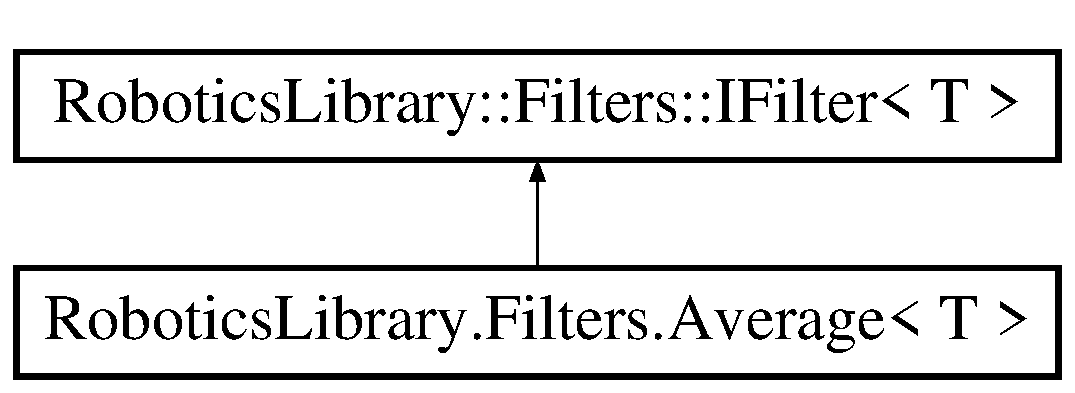
\includegraphics[height=2.000000cm]{d3/d9f/class_robotics_library_1_1_filters_1_1_average}
\end{center}
\end{figure}
\subsection*{Public Member Functions}
\begin{DoxyCompactItemize}
\item 
\hyperlink{class_robotics_library_1_1_filters_1_1_average_aa1f1ba91014e9fe0b966650b9ccbf514}{Average} (int \hyperlink{class_robotics_library_1_1_filters_1_1_average_a8db578c17df74d38278a0bcc18ca1d49}{Filter\+Count}=10)
\begin{DoxyCompactList}\small\item\em Construct an average filter with given roll-\/length. \end{DoxyCompactList}\item 
void \hyperlink{class_robotics_library_1_1_filters_1_1_average_a27479a3706425bb721a7694acd388cdd}{Feed} (T Input)
\begin{DoxyCompactList}\small\item\em Feeds a value into the filter. \end{DoxyCompactList}\item 
void \hyperlink{class_robotics_library_1_1_filters_1_1_average_a009ada38087402e4c8f5c3f3390123c8}{Feed} (T Input, T Rate)
\begin{DoxyCompactList}\small\item\em Feeds filter with specified rate. Not used for average filter. \end{DoxyCompactList}\end{DoxyCompactItemize}
\subsection*{Properties}
\begin{DoxyCompactItemize}
\item 
T \hyperlink{class_robotics_library_1_1_filters_1_1_average_aa59efec0916673c66b3507c4360c619e}{Output}\hspace{0.3cm}{\ttfamily  \mbox{[}get, private set\mbox{]}}
\end{DoxyCompactItemize}
\subsection*{Private Member Functions}
\begin{DoxyCompactItemize}
\item 
void \hyperlink{class_robotics_library_1_1_filters_1_1_average_af2d308005d9067a43cbb9968147b26dd}{Initialize\+Array} ()
\begin{DoxyCompactList}\small\item\em Initializes dynamic number array to all zeros.\end{DoxyCompactList}\end{DoxyCompactItemize}
\subsection*{Private Attributes}
\begin{DoxyCompactItemize}
\item 
dynamic \mbox{[}$\,$\mbox{]} \hyperlink{class_robotics_library_1_1_filters_1_1_average_abed97fe2d89a039ac76c7db768904fd5}{Average\+Array}
\item 
dynamic \hyperlink{class_robotics_library_1_1_filters_1_1_average_ab608142086c076a293b275fdfbfdf149}{Cur\+Sum}
\item 
int \hyperlink{class_robotics_library_1_1_filters_1_1_average_a8db578c17df74d38278a0bcc18ca1d49}{Filter\+Count}
\item 
int \hyperlink{class_robotics_library_1_1_filters_1_1_average_a22cecd8257b383616e9e581c5b61b3f5}{Index}
\item 
int \hyperlink{class_robotics_library_1_1_filters_1_1_average_a8ba4cd3fbcc9b94839a9a023c6b95732}{Iterations}
\end{DoxyCompactItemize}


\subsection{Detailed Description}
The \hyperlink{class_robotics_library_1_1_filters_1_1_average}{Average} filter is intended for use as an average-\/gathering system, using a rolling average with \char`\"{}roll-\/length\char`\"{} {\ttfamily Filter\+Count}.

Implementation Details\+:

$\ast$\+Construct \hyperlink{class_robotics_library_1_1_filters_1_1_average}{Average} filter given a rolling filter length, {\ttfamily Filter\+Count}

$\ast$\+Iteratively add values into the filter using {\ttfamily \hyperlink{class_robotics_library_1_1_filters_1_1_average_a27479a3706425bb721a7694acd388cdd}{Feed(\+T Input)}}

$\ast$\+Get the filter output by calling {\ttfamily Your\+Filter\+Instance.\+Output}


\begin{DoxyTemplParams}{Template Parameters}
{\em T} & A type, which must be a numeric.\\
\hline
\end{DoxyTemplParams}
\begin{Desc}
\item[Type Constraints]\begin{description}
\item[{\em T} : {\em I\+Comparable}]\end{description}
\end{Desc}


\subsection{Constructor \& Destructor Documentation}
\mbox{\Hypertarget{class_robotics_library_1_1_filters_1_1_average_aa1f1ba91014e9fe0b966650b9ccbf514}\label{class_robotics_library_1_1_filters_1_1_average_aa1f1ba91014e9fe0b966650b9ccbf514}} 
\index{Robotics\+Library\+::\+Filters\+::\+Average@{Robotics\+Library\+::\+Filters\+::\+Average}!Average@{Average}}
\index{Average@{Average}!Robotics\+Library\+::\+Filters\+::\+Average@{Robotics\+Library\+::\+Filters\+::\+Average}}
\subsubsection{\texorpdfstring{Average()}{Average()}}
{\footnotesize\ttfamily \hyperlink{class_robotics_library_1_1_filters_1_1_average}{Robotics\+Library.\+Filters.\+Average}$<$ T $>$.\hyperlink{class_robotics_library_1_1_filters_1_1_average}{Average} (\begin{DoxyParamCaption}\item[{int}]{Filter\+Count = {\ttfamily 10} }\end{DoxyParamCaption})}



Construct an average filter with given roll-\/length. 


\begin{DoxyParams}{Parameters}
{\em Filter\+Count} & Roll length for the average filter.\\
\hline
\end{DoxyParams}


\subsection{Member Function Documentation}
\mbox{\Hypertarget{class_robotics_library_1_1_filters_1_1_average_a27479a3706425bb721a7694acd388cdd}\label{class_robotics_library_1_1_filters_1_1_average_a27479a3706425bb721a7694acd388cdd}} 
\index{Robotics\+Library\+::\+Filters\+::\+Average@{Robotics\+Library\+::\+Filters\+::\+Average}!Feed@{Feed}}
\index{Feed@{Feed}!Robotics\+Library\+::\+Filters\+::\+Average@{Robotics\+Library\+::\+Filters\+::\+Average}}
\subsubsection{\texorpdfstring{Feed()}{Feed()}\hspace{0.1cm}{\footnotesize\ttfamily [1/2]}}
{\footnotesize\ttfamily void \hyperlink{class_robotics_library_1_1_filters_1_1_average}{Robotics\+Library.\+Filters.\+Average}$<$ T $>$.Feed (\begin{DoxyParamCaption}\item[{T}]{Input }\end{DoxyParamCaption})}



Feeds a value into the filter. 


\begin{DoxyParams}{Parameters}
{\em Input} & Value to feed into the filter.\\
\hline
\end{DoxyParams}


Implements \hyperlink{interface_robotics_library_1_1_filters_1_1_i_filter_a64855020add7b0354c2773696521c84e}{Robotics\+Library.\+Filters.\+I\+Filter$<$ T $>$}.

\mbox{\Hypertarget{class_robotics_library_1_1_filters_1_1_average_a009ada38087402e4c8f5c3f3390123c8}\label{class_robotics_library_1_1_filters_1_1_average_a009ada38087402e4c8f5c3f3390123c8}} 
\index{Robotics\+Library\+::\+Filters\+::\+Average@{Robotics\+Library\+::\+Filters\+::\+Average}!Feed@{Feed}}
\index{Feed@{Feed}!Robotics\+Library\+::\+Filters\+::\+Average@{Robotics\+Library\+::\+Filters\+::\+Average}}
\subsubsection{\texorpdfstring{Feed()}{Feed()}\hspace{0.1cm}{\footnotesize\ttfamily [2/2]}}
{\footnotesize\ttfamily void \hyperlink{class_robotics_library_1_1_filters_1_1_average}{Robotics\+Library.\+Filters.\+Average}$<$ T $>$.Feed (\begin{DoxyParamCaption}\item[{T}]{Input,  }\item[{T}]{Rate }\end{DoxyParamCaption})}



Feeds filter with specified rate. Not used for average filter. 


\begin{DoxyParams}{Parameters}
{\em Input} & Value to feed into the filer.\\
\hline
{\em Rate} & Current rate to feed into the filter.\\
\hline
\end{DoxyParams}


Implements \hyperlink{interface_robotics_library_1_1_filters_1_1_i_filter_a24d363fb2957923a256448e04634d9ca}{Robotics\+Library.\+Filters.\+I\+Filter$<$ T $>$}.

\mbox{\Hypertarget{class_robotics_library_1_1_filters_1_1_average_af2d308005d9067a43cbb9968147b26dd}\label{class_robotics_library_1_1_filters_1_1_average_af2d308005d9067a43cbb9968147b26dd}} 
\index{Robotics\+Library\+::\+Filters\+::\+Average@{Robotics\+Library\+::\+Filters\+::\+Average}!Initialize\+Array@{Initialize\+Array}}
\index{Initialize\+Array@{Initialize\+Array}!Robotics\+Library\+::\+Filters\+::\+Average@{Robotics\+Library\+::\+Filters\+::\+Average}}
\subsubsection{\texorpdfstring{Initialize\+Array()}{InitializeArray()}}
{\footnotesize\ttfamily void \hyperlink{class_robotics_library_1_1_filters_1_1_average}{Robotics\+Library.\+Filters.\+Average}$<$ T $>$.Initialize\+Array (\begin{DoxyParamCaption}{ }\end{DoxyParamCaption})\hspace{0.3cm}{\ttfamily [private]}}



Initializes dynamic number array to all zeros.



\subsection{Member Data Documentation}
\mbox{\Hypertarget{class_robotics_library_1_1_filters_1_1_average_abed97fe2d89a039ac76c7db768904fd5}\label{class_robotics_library_1_1_filters_1_1_average_abed97fe2d89a039ac76c7db768904fd5}} 
\index{Robotics\+Library\+::\+Filters\+::\+Average@{Robotics\+Library\+::\+Filters\+::\+Average}!Average\+Array@{Average\+Array}}
\index{Average\+Array@{Average\+Array}!Robotics\+Library\+::\+Filters\+::\+Average@{Robotics\+Library\+::\+Filters\+::\+Average}}
\subsubsection{\texorpdfstring{Average\+Array}{AverageArray}}
{\footnotesize\ttfamily dynamic \mbox{[}$\,$\mbox{]} \hyperlink{class_robotics_library_1_1_filters_1_1_average}{Robotics\+Library.\+Filters.\+Average}$<$ T $>$.Average\+Array\hspace{0.3cm}{\ttfamily [private]}}

\mbox{\Hypertarget{class_robotics_library_1_1_filters_1_1_average_ab608142086c076a293b275fdfbfdf149}\label{class_robotics_library_1_1_filters_1_1_average_ab608142086c076a293b275fdfbfdf149}} 
\index{Robotics\+Library\+::\+Filters\+::\+Average@{Robotics\+Library\+::\+Filters\+::\+Average}!Cur\+Sum@{Cur\+Sum}}
\index{Cur\+Sum@{Cur\+Sum}!Robotics\+Library\+::\+Filters\+::\+Average@{Robotics\+Library\+::\+Filters\+::\+Average}}
\subsubsection{\texorpdfstring{Cur\+Sum}{CurSum}}
{\footnotesize\ttfamily dynamic \hyperlink{class_robotics_library_1_1_filters_1_1_average}{Robotics\+Library.\+Filters.\+Average}$<$ T $>$.Cur\+Sum\hspace{0.3cm}{\ttfamily [private]}}

\mbox{\Hypertarget{class_robotics_library_1_1_filters_1_1_average_a8db578c17df74d38278a0bcc18ca1d49}\label{class_robotics_library_1_1_filters_1_1_average_a8db578c17df74d38278a0bcc18ca1d49}} 
\index{Robotics\+Library\+::\+Filters\+::\+Average@{Robotics\+Library\+::\+Filters\+::\+Average}!Filter\+Count@{Filter\+Count}}
\index{Filter\+Count@{Filter\+Count}!Robotics\+Library\+::\+Filters\+::\+Average@{Robotics\+Library\+::\+Filters\+::\+Average}}
\subsubsection{\texorpdfstring{Filter\+Count}{FilterCount}}
{\footnotesize\ttfamily int \hyperlink{class_robotics_library_1_1_filters_1_1_average}{Robotics\+Library.\+Filters.\+Average}$<$ T $>$.Filter\+Count\hspace{0.3cm}{\ttfamily [private]}}

\mbox{\Hypertarget{class_robotics_library_1_1_filters_1_1_average_a22cecd8257b383616e9e581c5b61b3f5}\label{class_robotics_library_1_1_filters_1_1_average_a22cecd8257b383616e9e581c5b61b3f5}} 
\index{Robotics\+Library\+::\+Filters\+::\+Average@{Robotics\+Library\+::\+Filters\+::\+Average}!Index@{Index}}
\index{Index@{Index}!Robotics\+Library\+::\+Filters\+::\+Average@{Robotics\+Library\+::\+Filters\+::\+Average}}
\subsubsection{\texorpdfstring{Index}{Index}}
{\footnotesize\ttfamily int \hyperlink{class_robotics_library_1_1_filters_1_1_average}{Robotics\+Library.\+Filters.\+Average}$<$ T $>$.Index\hspace{0.3cm}{\ttfamily [private]}}

\mbox{\Hypertarget{class_robotics_library_1_1_filters_1_1_average_a8ba4cd3fbcc9b94839a9a023c6b95732}\label{class_robotics_library_1_1_filters_1_1_average_a8ba4cd3fbcc9b94839a9a023c6b95732}} 
\index{Robotics\+Library\+::\+Filters\+::\+Average@{Robotics\+Library\+::\+Filters\+::\+Average}!Iterations@{Iterations}}
\index{Iterations@{Iterations}!Robotics\+Library\+::\+Filters\+::\+Average@{Robotics\+Library\+::\+Filters\+::\+Average}}
\subsubsection{\texorpdfstring{Iterations}{Iterations}}
{\footnotesize\ttfamily int \hyperlink{class_robotics_library_1_1_filters_1_1_average}{Robotics\+Library.\+Filters.\+Average}$<$ T $>$.Iterations\hspace{0.3cm}{\ttfamily [private]}}



\subsection{Property Documentation}
\mbox{\Hypertarget{class_robotics_library_1_1_filters_1_1_average_aa59efec0916673c66b3507c4360c619e}\label{class_robotics_library_1_1_filters_1_1_average_aa59efec0916673c66b3507c4360c619e}} 
\index{Robotics\+Library\+::\+Filters\+::\+Average@{Robotics\+Library\+::\+Filters\+::\+Average}!Output@{Output}}
\index{Output@{Output}!Robotics\+Library\+::\+Filters\+::\+Average@{Robotics\+Library\+::\+Filters\+::\+Average}}
\subsubsection{\texorpdfstring{Output}{Output}}
{\footnotesize\ttfamily T \hyperlink{class_robotics_library_1_1_filters_1_1_average}{Robotics\+Library.\+Filters.\+Average}$<$ T $>$.Output\hspace{0.3cm}{\ttfamily [get]}, {\ttfamily [private set]}}



The documentation for this class was generated from the following file\+:\begin{DoxyCompactItemize}
\item 
Filters/\hyperlink{_average_8cs}{Average.\+cs}\end{DoxyCompactItemize}

\hypertarget{class_robotics_library_1_1_commands_1_1_command}{}\section{Robotics\+Library.\+Commands.\+Command Class Reference}
\label{class_robotics_library_1_1_commands_1_1_command}\index{Robotics\+Library.\+Commands.\+Command@{Robotics\+Library.\+Commands.\+Command}}
\subsection*{Public Member Functions}
\begin{DoxyCompactItemize}
\item 
\hyperlink{class_robotics_library_1_1_commands_1_1_command_a1bfb451ce5eb9f1bbb5aa2b6a934e302}{Command} ()
\end{DoxyCompactItemize}


\subsection{Constructor \& Destructor Documentation}
\mbox{\Hypertarget{class_robotics_library_1_1_commands_1_1_command_a1bfb451ce5eb9f1bbb5aa2b6a934e302}\label{class_robotics_library_1_1_commands_1_1_command_a1bfb451ce5eb9f1bbb5aa2b6a934e302}} 
\index{Robotics\+Library\+::\+Commands\+::\+Command@{Robotics\+Library\+::\+Commands\+::\+Command}!Command@{Command}}
\index{Command@{Command}!Robotics\+Library\+::\+Commands\+::\+Command@{Robotics\+Library\+::\+Commands\+::\+Command}}
\subsubsection{\texorpdfstring{Command()}{Command()}}
{\footnotesize\ttfamily Robotics\+Library.\+Commands.\+Command.\+Command (\begin{DoxyParamCaption}{ }\end{DoxyParamCaption})}



The documentation for this class was generated from the following file\+:\begin{DoxyCompactItemize}
\item 
C\+:/\+Users/jaden/\+Documents/\+Git\+Hub/2017-\/18/science/\+Science Library/\+Commands/\hyperlink{_command_8cs}{Command.\+cs}\end{DoxyCompactItemize}

\hypertarget{class_robotics_library_1_1_communications_1_1_comm_handler}{}\section{Robotics\+Library.\+Communications.\+Comm\+Handler Class Reference}
\label{class_robotics_library_1_1_communications_1_1_comm_handler}\index{Robotics\+Library.\+Communications.\+Comm\+Handler@{Robotics\+Library.\+Communications.\+Comm\+Handler}}


Comms\+Handler handles communications send/receive including parsing information from source.  


\subsection*{Static Public Member Functions}
\begin{DoxyCompactItemize}
\item 
static bool \hyperlink{class_robotics_library_1_1_communications_1_1_comm_handler_a2c324044e0ecb019565eaa6d20fa0c27}{Start} (int Port=2024, float Cycle\+Time=0.\+02f, int Receive\+Buffer\+Size=64)
\begin{DoxyCompactList}\small\item\em Starts the \hyperlink{class_robotics_library_1_1_communications_1_1_comm_handler}{Comm\+Handler} \end{DoxyCompactList}\item 
static void \hyperlink{class_robotics_library_1_1_communications_1_1_comm_handler_aa49345cc033a788471167c08319e7af4}{Stop} ()
\begin{DoxyCompactList}\small\item\em Stops communications. \end{DoxyCompactList}\item 
static void \hyperlink{class_robotics_library_1_1_communications_1_1_comm_handler_a7e2e2f2de6d1272ab96507f17ee5e35c}{Restart} ()
\begin{DoxyCompactList}\small\item\em Use for restarting Comms. \end{DoxyCompactList}\item 
static void \hyperlink{class_robotics_library_1_1_communications_1_1_comm_handler_a9e875d4ed51f313878035fabb97f7c19}{Add\+Cycle\+Packet} (\hyperlink{class_robotics_library_1_1_communications_1_1_packet}{Packet} \hyperlink{class_robotics_library_1_1_communications_1_1_packet}{Packet})
\begin{DoxyCompactList}\small\item\em Adds packet to send buffer. \end{DoxyCompactList}\item 
static bool \hyperlink{class_robotics_library_1_1_communications_1_1_comm_handler_ac79d756af9d0a96058a2a26284591235}{Send\+Async\+Packet} (\hyperlink{class_robotics_library_1_1_communications_1_1_packet}{Packet} \hyperlink{class_robotics_library_1_1_communications_1_1_packet}{Packet})
\begin{DoxyCompactList}\small\item\em Sends a packet out of phase with the send cycles. \end{DoxyCompactList}\end{DoxyCompactItemize}
\subsection*{Static Private Member Functions}
\begin{DoxyCompactItemize}
\item 
static bool \hyperlink{class_robotics_library_1_1_communications_1_1_comm_handler_a1f6112825a07338045b07ba17a3e1d6b}{Initialize} ()
\begin{DoxyCompactList}\small\item\em Initializes \hyperlink{class_robotics_library_1_1_communications_1_1_comm_handler}{Comm\+Handler} (internal use only) \end{DoxyCompactList}\item 
static bool \hyperlink{class_robotics_library_1_1_communications_1_1_comm_handler_a0f3233960b73b33e8a94adef22fb9e2f}{Send\+Next\+Packet} ()
\begin{DoxyCompactList}\small\item\em Internal use only. Sends the next packet in the queue. \end{DoxyCompactList}\item 
static void \hyperlink{class_robotics_library_1_1_communications_1_1_comm_handler_a352403b8c19552676bb30cf55d54d8fb}{Send} ()
\begin{DoxyCompactList}\small\item\em Send loop start. Internal use only. Meant for threading. \end{DoxyCompactList}\item 
static void \hyperlink{class_robotics_library_1_1_communications_1_1_comm_handler_acae63122b382ab558378208db5e72680}{Receive} ()
\begin{DoxyCompactList}\small\item\em Receives messages and sends them to be parsed. \end{DoxyCompactList}\end{DoxyCompactItemize}
\subsection*{Static Private Attributes}
\begin{DoxyCompactItemize}
\item 
static Tcp\+Listener \hyperlink{class_robotics_library_1_1_communications_1_1_comm_handler_a1f06912e8a026624986cda6fa0d7f7ac}{Tcp\+Listener}
\item 
static I\+P\+End\+Point \hyperlink{class_robotics_library_1_1_communications_1_1_comm_handler_a9fdb1b92fa7ca7e35ffe8c474e41bfe9}{Endpoint}
\item 
static Queue$<$ \hyperlink{class_robotics_library_1_1_communications_1_1_packet}{Packet} $>$ \hyperlink{class_robotics_library_1_1_communications_1_1_comm_handler_acd3be385dfa108ad8d44fd2dee2560d8}{Send\+Queue}
\item 
static Thread \hyperlink{class_robotics_library_1_1_communications_1_1_comm_handler_af35ae76be97571d4e0ce17545a583552}{Send\+Thread}
\item 
static Thread \hyperlink{class_robotics_library_1_1_communications_1_1_comm_handler_afe2da330fb8f338d43af853fcb2bdfc7}{Receive\+Thread}
\item 
static float \hyperlink{class_robotics_library_1_1_communications_1_1_comm_handler_a8f90dd3c3703a0fad473842c2507a477}{Packet\+Interval\+Time}
\item 
static int \hyperlink{class_robotics_library_1_1_communications_1_1_comm_handler_a40a05621969ec969179a7f17eb2e64f3}{Receive\+Buffer\+Size}
\item 
static int \hyperlink{class_robotics_library_1_1_communications_1_1_comm_handler_a90a9510a5fb347278c41736032829323}{Port\+Number}
\item 
static bool \hyperlink{class_robotics_library_1_1_communications_1_1_comm_handler_a5a78eb290748121e4dfa9e8be8ed4077}{Continue}
\item 
static bool \hyperlink{class_robotics_library_1_1_communications_1_1_comm_handler_a29a665284d45e4c95b21055b5690b658}{Initialized}
\end{DoxyCompactItemize}


\subsection{Detailed Description}
Comms\+Handler handles communications send/receive including parsing information from source. 



\subsection{Member Function Documentation}
\mbox{\Hypertarget{class_robotics_library_1_1_communications_1_1_comm_handler_a9e875d4ed51f313878035fabb97f7c19}\label{class_robotics_library_1_1_communications_1_1_comm_handler_a9e875d4ed51f313878035fabb97f7c19}} 
\index{Robotics\+Library\+::\+Communications\+::\+Comm\+Handler@{Robotics\+Library\+::\+Communications\+::\+Comm\+Handler}!Add\+Cycle\+Packet@{Add\+Cycle\+Packet}}
\index{Add\+Cycle\+Packet@{Add\+Cycle\+Packet}!Robotics\+Library\+::\+Communications\+::\+Comm\+Handler@{Robotics\+Library\+::\+Communications\+::\+Comm\+Handler}}
\subsubsection{\texorpdfstring{Add\+Cycle\+Packet()}{AddCyclePacket()}}
{\footnotesize\ttfamily static void Robotics\+Library.\+Communications.\+Comm\+Handler.\+Add\+Cycle\+Packet (\begin{DoxyParamCaption}\item[{\hyperlink{class_robotics_library_1_1_communications_1_1_packet}{Packet}}]{Packet }\end{DoxyParamCaption})\hspace{0.3cm}{\ttfamily [static]}}



Adds packet to send buffer. 


\begin{DoxyParams}{Parameters}
{\em \hyperlink{class_robotics_library_1_1_communications_1_1_packet}{Packet}} & \hyperlink{class_robotics_library_1_1_communications_1_1_packet}{Packet} to add.\\
\hline
\end{DoxyParams}
\mbox{\Hypertarget{class_robotics_library_1_1_communications_1_1_comm_handler_a1f6112825a07338045b07ba17a3e1d6b}\label{class_robotics_library_1_1_communications_1_1_comm_handler_a1f6112825a07338045b07ba17a3e1d6b}} 
\index{Robotics\+Library\+::\+Communications\+::\+Comm\+Handler@{Robotics\+Library\+::\+Communications\+::\+Comm\+Handler}!Initialize@{Initialize}}
\index{Initialize@{Initialize}!Robotics\+Library\+::\+Communications\+::\+Comm\+Handler@{Robotics\+Library\+::\+Communications\+::\+Comm\+Handler}}
\subsubsection{\texorpdfstring{Initialize()}{Initialize()}}
{\footnotesize\ttfamily static bool Robotics\+Library.\+Communications.\+Comm\+Handler.\+Initialize (\begin{DoxyParamCaption}{ }\end{DoxyParamCaption})\hspace{0.3cm}{\ttfamily [static]}, {\ttfamily [private]}}



Initializes \hyperlink{class_robotics_library_1_1_communications_1_1_comm_handler}{Comm\+Handler} (internal use only) 

\begin{DoxyReturn}{Returns}
Returns whether or not initialization succeeded 
\end{DoxyReturn}
\mbox{\Hypertarget{class_robotics_library_1_1_communications_1_1_comm_handler_acae63122b382ab558378208db5e72680}\label{class_robotics_library_1_1_communications_1_1_comm_handler_acae63122b382ab558378208db5e72680}} 
\index{Robotics\+Library\+::\+Communications\+::\+Comm\+Handler@{Robotics\+Library\+::\+Communications\+::\+Comm\+Handler}!Receive@{Receive}}
\index{Receive@{Receive}!Robotics\+Library\+::\+Communications\+::\+Comm\+Handler@{Robotics\+Library\+::\+Communications\+::\+Comm\+Handler}}
\subsubsection{\texorpdfstring{Receive()}{Receive()}}
{\footnotesize\ttfamily static void Robotics\+Library.\+Communications.\+Comm\+Handler.\+Receive (\begin{DoxyParamCaption}{ }\end{DoxyParamCaption})\hspace{0.3cm}{\ttfamily [static]}, {\ttfamily [private]}}



Receives messages and sends them to be parsed. 

\mbox{\Hypertarget{class_robotics_library_1_1_communications_1_1_comm_handler_a7e2e2f2de6d1272ab96507f17ee5e35c}\label{class_robotics_library_1_1_communications_1_1_comm_handler_a7e2e2f2de6d1272ab96507f17ee5e35c}} 
\index{Robotics\+Library\+::\+Communications\+::\+Comm\+Handler@{Robotics\+Library\+::\+Communications\+::\+Comm\+Handler}!Restart@{Restart}}
\index{Restart@{Restart}!Robotics\+Library\+::\+Communications\+::\+Comm\+Handler@{Robotics\+Library\+::\+Communications\+::\+Comm\+Handler}}
\subsubsection{\texorpdfstring{Restart()}{Restart()}}
{\footnotesize\ttfamily static void Robotics\+Library.\+Communications.\+Comm\+Handler.\+Restart (\begin{DoxyParamCaption}{ }\end{DoxyParamCaption})\hspace{0.3cm}{\ttfamily [static]}}



Use for restarting Comms. 


\begin{DoxyItemize}
\item $\ast$ $\ast$ Important!! 
\end{DoxyItemize}\mbox{\Hypertarget{class_robotics_library_1_1_communications_1_1_comm_handler_a352403b8c19552676bb30cf55d54d8fb}\label{class_robotics_library_1_1_communications_1_1_comm_handler_a352403b8c19552676bb30cf55d54d8fb}} 
\index{Robotics\+Library\+::\+Communications\+::\+Comm\+Handler@{Robotics\+Library\+::\+Communications\+::\+Comm\+Handler}!Send@{Send}}
\index{Send@{Send}!Robotics\+Library\+::\+Communications\+::\+Comm\+Handler@{Robotics\+Library\+::\+Communications\+::\+Comm\+Handler}}
\subsubsection{\texorpdfstring{Send()}{Send()}}
{\footnotesize\ttfamily static void Robotics\+Library.\+Communications.\+Comm\+Handler.\+Send (\begin{DoxyParamCaption}{ }\end{DoxyParamCaption})\hspace{0.3cm}{\ttfamily [static]}, {\ttfamily [private]}}



Send loop start. Internal use only. Meant for threading. 

\mbox{\Hypertarget{class_robotics_library_1_1_communications_1_1_comm_handler_ac79d756af9d0a96058a2a26284591235}\label{class_robotics_library_1_1_communications_1_1_comm_handler_ac79d756af9d0a96058a2a26284591235}} 
\index{Robotics\+Library\+::\+Communications\+::\+Comm\+Handler@{Robotics\+Library\+::\+Communications\+::\+Comm\+Handler}!Send\+Async\+Packet@{Send\+Async\+Packet}}
\index{Send\+Async\+Packet@{Send\+Async\+Packet}!Robotics\+Library\+::\+Communications\+::\+Comm\+Handler@{Robotics\+Library\+::\+Communications\+::\+Comm\+Handler}}
\subsubsection{\texorpdfstring{Send\+Async\+Packet()}{SendAsyncPacket()}}
{\footnotesize\ttfamily static bool Robotics\+Library.\+Communications.\+Comm\+Handler.\+Send\+Async\+Packet (\begin{DoxyParamCaption}\item[{\hyperlink{class_robotics_library_1_1_communications_1_1_packet}{Packet}}]{Packet }\end{DoxyParamCaption})\hspace{0.3cm}{\ttfamily [static]}}



Sends a packet out of phase with the send cycles. 


\begin{DoxyParams}{Parameters}
{\em \hyperlink{class_robotics_library_1_1_communications_1_1_packet}{Packet}} & \hyperlink{class_robotics_library_1_1_communications_1_1_packet}{Packet} to send asynchronously\\
\hline
\end{DoxyParams}
\begin{DoxyReturn}{Returns}
Whether or not the send succeeded. 
\end{DoxyReturn}
\mbox{\Hypertarget{class_robotics_library_1_1_communications_1_1_comm_handler_a0f3233960b73b33e8a94adef22fb9e2f}\label{class_robotics_library_1_1_communications_1_1_comm_handler_a0f3233960b73b33e8a94adef22fb9e2f}} 
\index{Robotics\+Library\+::\+Communications\+::\+Comm\+Handler@{Robotics\+Library\+::\+Communications\+::\+Comm\+Handler}!Send\+Next\+Packet@{Send\+Next\+Packet}}
\index{Send\+Next\+Packet@{Send\+Next\+Packet}!Robotics\+Library\+::\+Communications\+::\+Comm\+Handler@{Robotics\+Library\+::\+Communications\+::\+Comm\+Handler}}
\subsubsection{\texorpdfstring{Send\+Next\+Packet()}{SendNextPacket()}}
{\footnotesize\ttfamily static bool Robotics\+Library.\+Communications.\+Comm\+Handler.\+Send\+Next\+Packet (\begin{DoxyParamCaption}{ }\end{DoxyParamCaption})\hspace{0.3cm}{\ttfamily [static]}, {\ttfamily [private]}}



Internal use only. Sends the next packet in the queue. 

\begin{DoxyReturn}{Returns}
Whether or not the send succeeded.
\end{DoxyReturn}
\mbox{\Hypertarget{class_robotics_library_1_1_communications_1_1_comm_handler_a2c324044e0ecb019565eaa6d20fa0c27}\label{class_robotics_library_1_1_communications_1_1_comm_handler_a2c324044e0ecb019565eaa6d20fa0c27}} 
\index{Robotics\+Library\+::\+Communications\+::\+Comm\+Handler@{Robotics\+Library\+::\+Communications\+::\+Comm\+Handler}!Start@{Start}}
\index{Start@{Start}!Robotics\+Library\+::\+Communications\+::\+Comm\+Handler@{Robotics\+Library\+::\+Communications\+::\+Comm\+Handler}}
\subsubsection{\texorpdfstring{Start()}{Start()}}
{\footnotesize\ttfamily static bool Robotics\+Library.\+Communications.\+Comm\+Handler.\+Start (\begin{DoxyParamCaption}\item[{int}]{Port = {\ttfamily 2024},  }\item[{float}]{Cycle\+Time = {\ttfamily 0.02f},  }\item[{int}]{Receive\+Buffer\+Size = {\ttfamily 64} }\end{DoxyParamCaption})\hspace{0.3cm}{\ttfamily [static]}}



Starts the \hyperlink{class_robotics_library_1_1_communications_1_1_comm_handler}{Comm\+Handler} 


\begin{DoxyParams}{Parameters}
{\em Port} & Port to listen on\\
\hline
{\em Cycle\+Time} & Minimum cycle time in between packet send/receive\\
\hline
{\em Receive\+Buffer\+Size} & Buffer receive size.\\
\hline
\end{DoxyParams}
\begin{DoxyReturn}{Returns}
Returns true is initialization succeeded, false otherwise. 
\end{DoxyReturn}
\mbox{\Hypertarget{class_robotics_library_1_1_communications_1_1_comm_handler_aa49345cc033a788471167c08319e7af4}\label{class_robotics_library_1_1_communications_1_1_comm_handler_aa49345cc033a788471167c08319e7af4}} 
\index{Robotics\+Library\+::\+Communications\+::\+Comm\+Handler@{Robotics\+Library\+::\+Communications\+::\+Comm\+Handler}!Stop@{Stop}}
\index{Stop@{Stop}!Robotics\+Library\+::\+Communications\+::\+Comm\+Handler@{Robotics\+Library\+::\+Communications\+::\+Comm\+Handler}}
\subsubsection{\texorpdfstring{Stop()}{Stop()}}
{\footnotesize\ttfamily static void Robotics\+Library.\+Communications.\+Comm\+Handler.\+Stop (\begin{DoxyParamCaption}{ }\end{DoxyParamCaption})\hspace{0.3cm}{\ttfamily [static]}}



Stops communications. 



\subsection{Member Data Documentation}
\mbox{\Hypertarget{class_robotics_library_1_1_communications_1_1_comm_handler_a5a78eb290748121e4dfa9e8be8ed4077}\label{class_robotics_library_1_1_communications_1_1_comm_handler_a5a78eb290748121e4dfa9e8be8ed4077}} 
\index{Robotics\+Library\+::\+Communications\+::\+Comm\+Handler@{Robotics\+Library\+::\+Communications\+::\+Comm\+Handler}!Continue@{Continue}}
\index{Continue@{Continue}!Robotics\+Library\+::\+Communications\+::\+Comm\+Handler@{Robotics\+Library\+::\+Communications\+::\+Comm\+Handler}}
\subsubsection{\texorpdfstring{Continue}{Continue}}
{\footnotesize\ttfamily bool Robotics\+Library.\+Communications.\+Comm\+Handler.\+Continue\hspace{0.3cm}{\ttfamily [static]}, {\ttfamily [private]}}

\mbox{\Hypertarget{class_robotics_library_1_1_communications_1_1_comm_handler_a9fdb1b92fa7ca7e35ffe8c474e41bfe9}\label{class_robotics_library_1_1_communications_1_1_comm_handler_a9fdb1b92fa7ca7e35ffe8c474e41bfe9}} 
\index{Robotics\+Library\+::\+Communications\+::\+Comm\+Handler@{Robotics\+Library\+::\+Communications\+::\+Comm\+Handler}!Endpoint@{Endpoint}}
\index{Endpoint@{Endpoint}!Robotics\+Library\+::\+Communications\+::\+Comm\+Handler@{Robotics\+Library\+::\+Communications\+::\+Comm\+Handler}}
\subsubsection{\texorpdfstring{Endpoint}{Endpoint}}
{\footnotesize\ttfamily I\+P\+End\+Point Robotics\+Library.\+Communications.\+Comm\+Handler.\+Endpoint\hspace{0.3cm}{\ttfamily [static]}, {\ttfamily [private]}}

\mbox{\Hypertarget{class_robotics_library_1_1_communications_1_1_comm_handler_a29a665284d45e4c95b21055b5690b658}\label{class_robotics_library_1_1_communications_1_1_comm_handler_a29a665284d45e4c95b21055b5690b658}} 
\index{Robotics\+Library\+::\+Communications\+::\+Comm\+Handler@{Robotics\+Library\+::\+Communications\+::\+Comm\+Handler}!Initialized@{Initialized}}
\index{Initialized@{Initialized}!Robotics\+Library\+::\+Communications\+::\+Comm\+Handler@{Robotics\+Library\+::\+Communications\+::\+Comm\+Handler}}
\subsubsection{\texorpdfstring{Initialized}{Initialized}}
{\footnotesize\ttfamily bool Robotics\+Library.\+Communications.\+Comm\+Handler.\+Initialized\hspace{0.3cm}{\ttfamily [static]}, {\ttfamily [private]}}

\mbox{\Hypertarget{class_robotics_library_1_1_communications_1_1_comm_handler_a8f90dd3c3703a0fad473842c2507a477}\label{class_robotics_library_1_1_communications_1_1_comm_handler_a8f90dd3c3703a0fad473842c2507a477}} 
\index{Robotics\+Library\+::\+Communications\+::\+Comm\+Handler@{Robotics\+Library\+::\+Communications\+::\+Comm\+Handler}!Packet\+Interval\+Time@{Packet\+Interval\+Time}}
\index{Packet\+Interval\+Time@{Packet\+Interval\+Time}!Robotics\+Library\+::\+Communications\+::\+Comm\+Handler@{Robotics\+Library\+::\+Communications\+::\+Comm\+Handler}}
\subsubsection{\texorpdfstring{Packet\+Interval\+Time}{PacketIntervalTime}}
{\footnotesize\ttfamily float Robotics\+Library.\+Communications.\+Comm\+Handler.\+Packet\+Interval\+Time\hspace{0.3cm}{\ttfamily [static]}, {\ttfamily [private]}}

\mbox{\Hypertarget{class_robotics_library_1_1_communications_1_1_comm_handler_a90a9510a5fb347278c41736032829323}\label{class_robotics_library_1_1_communications_1_1_comm_handler_a90a9510a5fb347278c41736032829323}} 
\index{Robotics\+Library\+::\+Communications\+::\+Comm\+Handler@{Robotics\+Library\+::\+Communications\+::\+Comm\+Handler}!Port\+Number@{Port\+Number}}
\index{Port\+Number@{Port\+Number}!Robotics\+Library\+::\+Communications\+::\+Comm\+Handler@{Robotics\+Library\+::\+Communications\+::\+Comm\+Handler}}
\subsubsection{\texorpdfstring{Port\+Number}{PortNumber}}
{\footnotesize\ttfamily int Robotics\+Library.\+Communications.\+Comm\+Handler.\+Port\+Number\hspace{0.3cm}{\ttfamily [static]}, {\ttfamily [private]}}

\mbox{\Hypertarget{class_robotics_library_1_1_communications_1_1_comm_handler_a40a05621969ec969179a7f17eb2e64f3}\label{class_robotics_library_1_1_communications_1_1_comm_handler_a40a05621969ec969179a7f17eb2e64f3}} 
\index{Robotics\+Library\+::\+Communications\+::\+Comm\+Handler@{Robotics\+Library\+::\+Communications\+::\+Comm\+Handler}!Receive\+Buffer\+Size@{Receive\+Buffer\+Size}}
\index{Receive\+Buffer\+Size@{Receive\+Buffer\+Size}!Robotics\+Library\+::\+Communications\+::\+Comm\+Handler@{Robotics\+Library\+::\+Communications\+::\+Comm\+Handler}}
\subsubsection{\texorpdfstring{Receive\+Buffer\+Size}{ReceiveBufferSize}}
{\footnotesize\ttfamily int Robotics\+Library.\+Communications.\+Comm\+Handler.\+Receive\+Buffer\+Size\hspace{0.3cm}{\ttfamily [static]}, {\ttfamily [private]}}

\mbox{\Hypertarget{class_robotics_library_1_1_communications_1_1_comm_handler_afe2da330fb8f338d43af853fcb2bdfc7}\label{class_robotics_library_1_1_communications_1_1_comm_handler_afe2da330fb8f338d43af853fcb2bdfc7}} 
\index{Robotics\+Library\+::\+Communications\+::\+Comm\+Handler@{Robotics\+Library\+::\+Communications\+::\+Comm\+Handler}!Receive\+Thread@{Receive\+Thread}}
\index{Receive\+Thread@{Receive\+Thread}!Robotics\+Library\+::\+Communications\+::\+Comm\+Handler@{Robotics\+Library\+::\+Communications\+::\+Comm\+Handler}}
\subsubsection{\texorpdfstring{Receive\+Thread}{ReceiveThread}}
{\footnotesize\ttfamily Thread Robotics\+Library.\+Communications.\+Comm\+Handler.\+Receive\+Thread\hspace{0.3cm}{\ttfamily [static]}, {\ttfamily [private]}}

\mbox{\Hypertarget{class_robotics_library_1_1_communications_1_1_comm_handler_acd3be385dfa108ad8d44fd2dee2560d8}\label{class_robotics_library_1_1_communications_1_1_comm_handler_acd3be385dfa108ad8d44fd2dee2560d8}} 
\index{Robotics\+Library\+::\+Communications\+::\+Comm\+Handler@{Robotics\+Library\+::\+Communications\+::\+Comm\+Handler}!Send\+Queue@{Send\+Queue}}
\index{Send\+Queue@{Send\+Queue}!Robotics\+Library\+::\+Communications\+::\+Comm\+Handler@{Robotics\+Library\+::\+Communications\+::\+Comm\+Handler}}
\subsubsection{\texorpdfstring{Send\+Queue}{SendQueue}}
{\footnotesize\ttfamily Queue$<$\hyperlink{class_robotics_library_1_1_communications_1_1_packet}{Packet}$>$ Robotics\+Library.\+Communications.\+Comm\+Handler.\+Send\+Queue\hspace{0.3cm}{\ttfamily [static]}, {\ttfamily [private]}}

\mbox{\Hypertarget{class_robotics_library_1_1_communications_1_1_comm_handler_af35ae76be97571d4e0ce17545a583552}\label{class_robotics_library_1_1_communications_1_1_comm_handler_af35ae76be97571d4e0ce17545a583552}} 
\index{Robotics\+Library\+::\+Communications\+::\+Comm\+Handler@{Robotics\+Library\+::\+Communications\+::\+Comm\+Handler}!Send\+Thread@{Send\+Thread}}
\index{Send\+Thread@{Send\+Thread}!Robotics\+Library\+::\+Communications\+::\+Comm\+Handler@{Robotics\+Library\+::\+Communications\+::\+Comm\+Handler}}
\subsubsection{\texorpdfstring{Send\+Thread}{SendThread}}
{\footnotesize\ttfamily Thread Robotics\+Library.\+Communications.\+Comm\+Handler.\+Send\+Thread\hspace{0.3cm}{\ttfamily [static]}, {\ttfamily [private]}}

\mbox{\Hypertarget{class_robotics_library_1_1_communications_1_1_comm_handler_a1f06912e8a026624986cda6fa0d7f7ac}\label{class_robotics_library_1_1_communications_1_1_comm_handler_a1f06912e8a026624986cda6fa0d7f7ac}} 
\index{Robotics\+Library\+::\+Communications\+::\+Comm\+Handler@{Robotics\+Library\+::\+Communications\+::\+Comm\+Handler}!Tcp\+Listener@{Tcp\+Listener}}
\index{Tcp\+Listener@{Tcp\+Listener}!Robotics\+Library\+::\+Communications\+::\+Comm\+Handler@{Robotics\+Library\+::\+Communications\+::\+Comm\+Handler}}
\subsubsection{\texorpdfstring{Tcp\+Listener}{TcpListener}}
{\footnotesize\ttfamily Tcp\+Listener Robotics\+Library.\+Communications.\+Comm\+Handler.\+Tcp\+Listener\hspace{0.3cm}{\ttfamily [static]}, {\ttfamily [private]}}



The documentation for this class was generated from the following file\+:\begin{DoxyCompactItemize}
\item 
Communications/\hyperlink{_comm_handler_8cs}{Comm\+Handler.\+cs}\end{DoxyCompactItemize}

\hypertarget{class_robotics_library_1_1_errors_1_1_error_handler}{}\section{Robotics\+Library.\+Errors.\+Error\+Handler Class Reference}
\label{class_robotics_library_1_1_errors_1_1_error_handler}\index{Robotics\+Library.\+Errors.\+Error\+Handler@{Robotics\+Library.\+Errors.\+Error\+Handler}}


Handles\+:  


\subsection*{Static Public Member Functions}
\begin{DoxyCompactItemize}
\item 
static void \hyperlink{class_robotics_library_1_1_errors_1_1_error_handler_a3a4b2937527bf41cc34d4d244c20364c}{Throw} (Exception e, bool Send=true)
\begin{DoxyCompactList}\small\item\em Throws and error given an exception. \end{DoxyCompactList}\item 
static void \hyperlink{class_robotics_library_1_1_errors_1_1_error_handler_a3d2861114cd4e8cc38cd8c5a8c539a0e}{Throw} (int Error, bool Send=true)
\begin{DoxyCompactList}\small\item\em Throws an error given an integer value for the exception. \end{DoxyCompactList}\end{DoxyCompactItemize}


\subsection{Detailed Description}
Handles\+: 


\begin{DoxyItemize}
\item On board error throwing
\item Throwing errors over comms
\begin{DoxyItemize}
\item Whether or not error is sent over comms is determined by the boolean {\ttfamily Send}. 
\end{DoxyItemize}
\end{DoxyItemize}

\subsection{Member Function Documentation}
\mbox{\Hypertarget{class_robotics_library_1_1_errors_1_1_error_handler_a3a4b2937527bf41cc34d4d244c20364c}\label{class_robotics_library_1_1_errors_1_1_error_handler_a3a4b2937527bf41cc34d4d244c20364c}} 
\index{Robotics\+Library\+::\+Errors\+::\+Error\+Handler@{Robotics\+Library\+::\+Errors\+::\+Error\+Handler}!Throw@{Throw}}
\index{Throw@{Throw}!Robotics\+Library\+::\+Errors\+::\+Error\+Handler@{Robotics\+Library\+::\+Errors\+::\+Error\+Handler}}
\subsubsection{\texorpdfstring{Throw()}{Throw()}\hspace{0.1cm}{\footnotesize\ttfamily [1/2]}}
{\footnotesize\ttfamily static void Robotics\+Library.\+Errors.\+Error\+Handler.\+Throw (\begin{DoxyParamCaption}\item[{Exception}]{e,  }\item[{bool}]{Send = {\ttfamily true} }\end{DoxyParamCaption})\hspace{0.3cm}{\ttfamily [static]}}



Throws and error given an exception. 


\begin{DoxyParams}{Parameters}
{\em e} & Exception to throw as an error.\\
\hline
{\em Send} & true if Error to be sent over comms.\\
\hline
\end{DoxyParams}
\mbox{\Hypertarget{class_robotics_library_1_1_errors_1_1_error_handler_a3d2861114cd4e8cc38cd8c5a8c539a0e}\label{class_robotics_library_1_1_errors_1_1_error_handler_a3d2861114cd4e8cc38cd8c5a8c539a0e}} 
\index{Robotics\+Library\+::\+Errors\+::\+Error\+Handler@{Robotics\+Library\+::\+Errors\+::\+Error\+Handler}!Throw@{Throw}}
\index{Throw@{Throw}!Robotics\+Library\+::\+Errors\+::\+Error\+Handler@{Robotics\+Library\+::\+Errors\+::\+Error\+Handler}}
\subsubsection{\texorpdfstring{Throw()}{Throw()}\hspace{0.1cm}{\footnotesize\ttfamily [2/2]}}
{\footnotesize\ttfamily static void Robotics\+Library.\+Errors.\+Error\+Handler.\+Throw (\begin{DoxyParamCaption}\item[{int}]{Error,  }\item[{bool}]{Send = {\ttfamily true} }\end{DoxyParamCaption})\hspace{0.3cm}{\ttfamily [static]}}



Throws an error given an integer value for the exception. 


\begin{DoxyParams}{Parameters}
{\em Error} & The integer value of the error to throw\\
\hline
{\em Send} & true if Error to be send over comms.\\
\hline
\end{DoxyParams}


The documentation for this class was generated from the following file\+:\begin{DoxyCompactItemize}
\item 
Errors/\hyperlink{_error_handler_8cs}{Error\+Handler.\+cs}\end{DoxyCompactItemize}

\hypertarget{interface_robotics_library_1_1_filters_1_1_i_filter}{}\section{Robotics\+Library.\+Filters.\+I\+Filter$<$ T $>$ Interface Template Reference}
\label{interface_robotics_library_1_1_filters_1_1_i_filter}\index{Robotics\+Library.\+Filters.\+I\+Filter$<$ T $>$@{Robotics\+Library.\+Filters.\+I\+Filter$<$ T $>$}}


F\+I\+L\+T\+ER \hyperlink{_filter_8cs}{Filter.\+cs} Written by Jaden Bottemiller May 31, 2017  


Inheritance diagram for Robotics\+Library.\+Filters.\+I\+Filter$<$ T $>$\+:\begin{figure}[H]
\begin{center}
\leavevmode
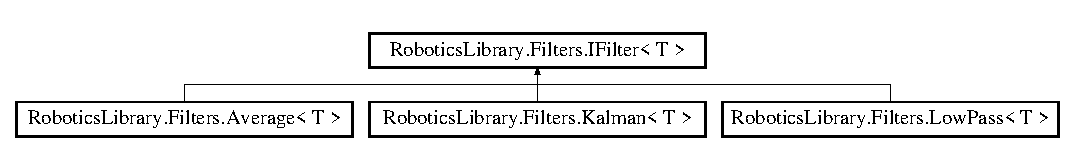
\includegraphics[height=1.602289cm]{interface_robotics_library_1_1_filters_1_1_i_filter}
\end{center}
\end{figure}
\subsection*{Public Member Functions}
\begin{DoxyCompactItemize}
\item 
void \hyperlink{interface_robotics_library_1_1_filters_1_1_i_filter_a24d363fb2957923a256448e04634d9ca}{Feed} (T Input, T Rate)
\item 
void \hyperlink{interface_robotics_library_1_1_filters_1_1_i_filter_a64855020add7b0354c2773696521c84e}{Feed} (T Input)
\end{DoxyCompactItemize}


\subsection{Detailed Description}
F\+I\+L\+T\+ER \hyperlink{_filter_8cs}{Filter.\+cs} Written by Jaden Bottemiller May 31, 2017 

Unit testing took place on\+: \mbox{[} N\+OT Y\+ET \mbox{]}

This is an interface meant to wrap all filters in the \hyperlink{namespace_robotics_library_1_1_filters}{Filters} namespace.


\begin{DoxyItemize}
\item $\ast$ $\ast$ \hyperlink{namespace_robotics_library_1_1_filters}{Filters} requires the Robotics\+Library.\+Utility Namespace.
\item $\ast$ $\ast$ Some \hyperlink{namespace_robotics_library_1_1_filters}{Filters} require use of just the \hyperlink{interface_robotics_library_1_1_filters_1_1_i_filter_a64855020add7b0354c2773696521c84e}{Feed(\+T Input)} method. Others require a given \hyperlink{interface_robotics_library_1_1_filters_1_1_i_filter_a24d363fb2957923a256448e04634d9ca}{Feed(\+T Input, T Rate)}. See the documentation for the given filter to determine necessary information. 
\end{DoxyItemize}\begin{Desc}
\item[Type Constraints]\begin{description}
\item[{\em T} : {\em I\+Comparable}]\end{description}
\end{Desc}


\subsection{Member Function Documentation}
\mbox{\Hypertarget{interface_robotics_library_1_1_filters_1_1_i_filter_a24d363fb2957923a256448e04634d9ca}\label{interface_robotics_library_1_1_filters_1_1_i_filter_a24d363fb2957923a256448e04634d9ca}} 
\index{Robotics\+Library\+::\+Filters\+::\+I\+Filter@{Robotics\+Library\+::\+Filters\+::\+I\+Filter}!Feed@{Feed}}
\index{Feed@{Feed}!Robotics\+Library\+::\+Filters\+::\+I\+Filter@{Robotics\+Library\+::\+Filters\+::\+I\+Filter}}
\subsubsection{\texorpdfstring{Feed()}{Feed()}\hspace{0.1cm}{\footnotesize\ttfamily [1/2]}}
{\footnotesize\ttfamily void \hyperlink{interface_robotics_library_1_1_filters_1_1_i_filter}{Robotics\+Library.\+Filters.\+I\+Filter}$<$ T $>$.Feed (\begin{DoxyParamCaption}\item[{T}]{Input,  }\item[{T}]{Rate }\end{DoxyParamCaption})}



Implemented in \hyperlink{class_robotics_library_1_1_filters_1_1_kalman_a5c2f27a6d48ede3369d4b9ac776954db}{Robotics\+Library.\+Filters.\+Kalman$<$ T $>$}, \hyperlink{class_robotics_library_1_1_filters_1_1_average_a009ada38087402e4c8f5c3f3390123c8}{Robotics\+Library.\+Filters.\+Average$<$ T $>$}, and \hyperlink{class_robotics_library_1_1_filters_1_1_low_pass_a9b8d610c0f54a17e84ea5e9252c9e215}{Robotics\+Library.\+Filters.\+Low\+Pass$<$ T $>$}.

\mbox{\Hypertarget{interface_robotics_library_1_1_filters_1_1_i_filter_a64855020add7b0354c2773696521c84e}\label{interface_robotics_library_1_1_filters_1_1_i_filter_a64855020add7b0354c2773696521c84e}} 
\index{Robotics\+Library\+::\+Filters\+::\+I\+Filter@{Robotics\+Library\+::\+Filters\+::\+I\+Filter}!Feed@{Feed}}
\index{Feed@{Feed}!Robotics\+Library\+::\+Filters\+::\+I\+Filter@{Robotics\+Library\+::\+Filters\+::\+I\+Filter}}
\subsubsection{\texorpdfstring{Feed()}{Feed()}\hspace{0.1cm}{\footnotesize\ttfamily [2/2]}}
{\footnotesize\ttfamily void \hyperlink{interface_robotics_library_1_1_filters_1_1_i_filter}{Robotics\+Library.\+Filters.\+I\+Filter}$<$ T $>$.Feed (\begin{DoxyParamCaption}\item[{T}]{Input }\end{DoxyParamCaption})}



Implemented in \hyperlink{class_robotics_library_1_1_filters_1_1_kalman_a92a029a73d197e692fc35b1f6e0ba238}{Robotics\+Library.\+Filters.\+Kalman$<$ T $>$}, \hyperlink{class_robotics_library_1_1_filters_1_1_average_a27479a3706425bb721a7694acd388cdd}{Robotics\+Library.\+Filters.\+Average$<$ T $>$}, and \hyperlink{class_robotics_library_1_1_filters_1_1_low_pass_adba4c542b4935845404729ebb2222b72}{Robotics\+Library.\+Filters.\+Low\+Pass$<$ T $>$}.



The documentation for this interface was generated from the following file\+:\begin{DoxyCompactItemize}
\item 
Filters/\hyperlink{_filter_8cs}{Filter.\+cs}\end{DoxyCompactItemize}

\hypertarget{class_robotics_library_1_1_filters_1_1_kalman}{}\section{Robotics\+Library.\+Filters.\+Kalman$<$ T $>$ Class Template Reference}
\label{class_robotics_library_1_1_filters_1_1_kalman}\index{Robotics\+Library.\+Filters.\+Kalman$<$ T $>$@{Robotics\+Library.\+Filters.\+Kalman$<$ T $>$}}


This \hyperlink{class_robotics_library_1_1_filters_1_1_kalman}{Kalman} Filter class is intended to be used for the implementation of a single-\/measurement \hyperlink{class_robotics_library_1_1_filters_1_1_kalman}{Kalman} Filter. See \href{https://en.m.wikipedia.org/wiki/Kalman_filter}{\tt https\+://en.\+m.\+wikipedia.\+org/wiki/\+Kalman\+\_\+filter} for details of the construction and operation of a \hyperlink{class_robotics_library_1_1_filters_1_1_kalman}{Kalman} filter. 


Inheritance diagram for Robotics\+Library.\+Filters.\+Kalman$<$ T $>$\+:\begin{figure}[H]
\begin{center}
\leavevmode
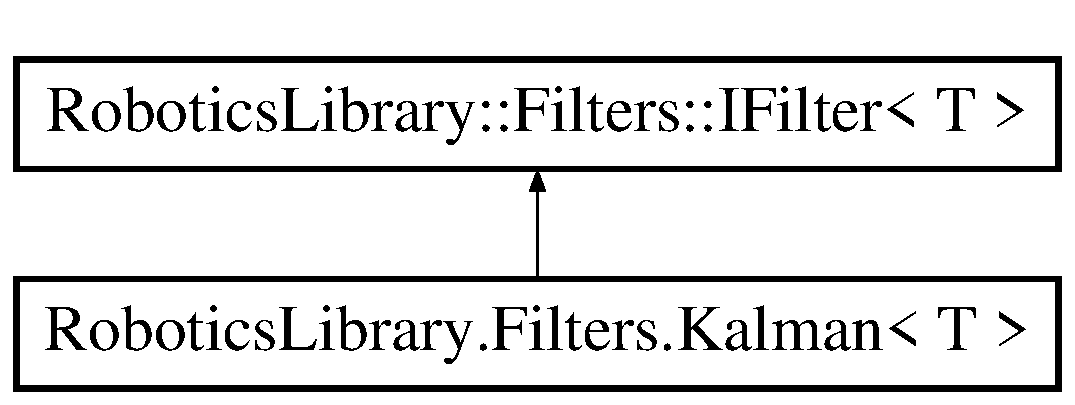
\includegraphics[height=2.000000cm]{d8/d85/class_robotics_library_1_1_filters_1_1_kalman}
\end{center}
\end{figure}
\subsection*{Public Member Functions}
\begin{DoxyCompactItemize}
\item 
\hyperlink{class_robotics_library_1_1_filters_1_1_kalman_a4c97ac8d96d0ce247be5331d549ff8df}{Kalman} ()
\begin{DoxyCompactList}\small\item\em Handles construction of the \hyperlink{class_robotics_library_1_1_filters_1_1_kalman}{Kalman} filter with default filter coefficients. See class comment for more information regarding implementation.\end{DoxyCompactList}\item 
void \hyperlink{class_robotics_library_1_1_filters_1_1_kalman_a92a029a73d197e692fc35b1f6e0ba238}{Feed} (T Input)
\begin{DoxyCompactList}\small\item\em Feeds the \hyperlink{class_robotics_library_1_1_filters_1_1_kalman}{Kalman} filter with an input, but only uses the last supplied rate.\end{DoxyCompactList}\item 
void \hyperlink{class_robotics_library_1_1_filters_1_1_kalman_aec1fb77c692d3d444d1cbd60f2b2592c}{Initialize} ()
\begin{DoxyCompactList}\small\item\em Initializes the \hyperlink{class_robotics_library_1_1_filters_1_1_kalman}{Kalman} filter. Call before running iteratively.\end{DoxyCompactList}\item 
void \hyperlink{class_robotics_library_1_1_filters_1_1_kalman_a5c2f27a6d48ede3369d4b9ac776954db}{Feed} (T Input, T Rate)
\begin{DoxyCompactList}\small\item\em Feeds the \hyperlink{class_robotics_library_1_1_filters_1_1_kalman}{Kalman} filter with an input and rate and calculates the feedback from the filter.\end{DoxyCompactList}\end{DoxyCompactItemize}
\subsection*{Public Attributes}
\begin{DoxyCompactItemize}
\item 
double \hyperlink{class_robotics_library_1_1_filters_1_1_kalman_a99ad42967bc86d34d72dfac39fa83a56}{Q}
\item 
double \hyperlink{class_robotics_library_1_1_filters_1_1_kalman_ac8d5e6103a05524967572e38492b6ea9}{Qbias}
\end{DoxyCompactItemize}
\subsection*{Properties}
\begin{DoxyCompactItemize}
\item 
double \hyperlink{class_robotics_library_1_1_filters_1_1_kalman_abb21b31283beac465da9fe1c947a52cf}{Rmeasure}\hspace{0.3cm}{\ttfamily  \mbox{[}get, set\mbox{]}}
\item 
T \hyperlink{class_robotics_library_1_1_filters_1_1_kalman_af2e026fe76f5a30e8da58dcc654ec26d}{Output}\hspace{0.3cm}{\ttfamily  \mbox{[}get, private set\mbox{]}}
\item 
bool \hyperlink{class_robotics_library_1_1_filters_1_1_kalman_a3c9aa0e2650a8085161821e858e64bb9}{Initialized}\hspace{0.3cm}{\ttfamily  \mbox{[}get, private set\mbox{]}}
\end{DoxyCompactItemize}
\subsection*{Private Attributes}
\begin{DoxyCompactItemize}
\item 
double \hyperlink{class_robotics_library_1_1_filters_1_1_kalman_a6af091d7f8b91835dfc8d4249de67db9}{Calc\+Measure}
\item 
double \hyperlink{class_robotics_library_1_1_filters_1_1_kalman_a9ab33a9815f641e2867562bc87c4903b}{Bias}
\item 
double \hyperlink{class_robotics_library_1_1_filters_1_1_kalman_a3460c72ca1559167bdc75b15af62f02d}{New\+Rate}
\item 
double \hyperlink{class_robotics_library_1_1_filters_1_1_kalman_aa64729ed425d53ec193cce9eb533bdc5}{Y}
\item 
double \hyperlink{class_robotics_library_1_1_filters_1_1_kalman_a66d8ab98513fe6152b81ad8cb5019240}{S}
\item 
double \mbox{[},\mbox{]} \hyperlink{class_robotics_library_1_1_filters_1_1_kalman_aeebdcb0526a88f010d3f703b137da9b8}{P}
\item 
double \mbox{[}$\,$\mbox{]} \hyperlink{class_robotics_library_1_1_filters_1_1_kalman_acfc2b088052cf66ad450dadac5a447dc}{K}
\item 
T \hyperlink{class_robotics_library_1_1_filters_1_1_kalman_a87b556d80535f21c00bf1dd7235c5953}{Last\+Rate}
\item 
Stopwatch \hyperlink{class_robotics_library_1_1_filters_1_1_kalman_a849c2e4310b17b9fe3d63d14fc29b325}{Stop\+Watch}
\item 
double \hyperlink{class_robotics_library_1_1_filters_1_1_kalman_a0ef91e55c642e8c6b69093ab955f4b5e}{Last\+Time}
\end{DoxyCompactItemize}


\subsection{Detailed Description}
This \hyperlink{class_robotics_library_1_1_filters_1_1_kalman}{Kalman} Filter class is intended to be used for the implementation of a single-\/measurement \hyperlink{class_robotics_library_1_1_filters_1_1_kalman}{Kalman} Filter. See \href{https://en.m.wikipedia.org/wiki/Kalman_filter}{\tt https\+://en.\+m.\+wikipedia.\+org/wiki/\+Kalman\+\_\+filter} for details of the construction and operation of a \hyperlink{class_robotics_library_1_1_filters_1_1_kalman}{Kalman} filter.


\begin{DoxyTemplParams}{Template Parameters}
{\em T} & A type, which must be a numeric.\\
\hline
\end{DoxyTemplParams}


Basic implementation as follows\+:

For basic prototyping, it is probably best to leave the coefficients as their defaults. For tuning, you can change the coefficients later.

Coefficients\+: {\ttfamily  Q,}{\ttfamily  Qbias, }{\ttfamily  Rmeasure}.


\begin{DoxyItemize}
\item Before iterations call {\ttfamily \hyperlink{class_robotics_library_1_1_filters_1_1_kalman_aec1fb77c692d3d444d1cbd60f2b2592c}{Initialize()}}
\item Iteratively call {\ttfamily  \hyperlink{class_robotics_library_1_1_filters_1_1_kalman_a5c2f27a6d48ede3369d4b9ac776954db}{Feed(\+T input, T rate)}} (This is important because the filter is time-\/dependent)
\item To get the value returned from the filter, call\+: {\ttfamily  Your\+Kalman\+Filter\+Instance.\+Ouput } $\ast$$\ast$$\ast$$\ast$$\ast$ I\+M\+P\+O\+R\+T\+A\+NT $\ast$$\ast$$\ast$$\ast$$\ast$
\end{DoxyItemize}

" \hyperlink{class_robotics_library_1_1_filters_1_1_kalman}{Kalman} filters produce the optimal estimate for a linear system. As such, a sensor or system must have (or be close to) a linear response in order to apply a \hyperlink{class_robotics_library_1_1_filters_1_1_kalman}{Kalman} filter. " Quote from\+: \href{http://robotsforroboticists.com/kalman-filtering/}{\tt http\+://robotsforroboticists.\+com/kalman-\/filtering/} \begin{Desc}
\item[Type Constraints]\begin{description}
\item[{\em T} : {\em I\+Comparable}]\end{description}
\end{Desc}


\subsection{Constructor \& Destructor Documentation}
\mbox{\Hypertarget{class_robotics_library_1_1_filters_1_1_kalman_a4c97ac8d96d0ce247be5331d549ff8df}\label{class_robotics_library_1_1_filters_1_1_kalman_a4c97ac8d96d0ce247be5331d549ff8df}} 
\index{Robotics\+Library\+::\+Filters\+::\+Kalman@{Robotics\+Library\+::\+Filters\+::\+Kalman}!Kalman@{Kalman}}
\index{Kalman@{Kalman}!Robotics\+Library\+::\+Filters\+::\+Kalman@{Robotics\+Library\+::\+Filters\+::\+Kalman}}
\subsubsection{\texorpdfstring{Kalman()}{Kalman()}}
{\footnotesize\ttfamily \hyperlink{class_robotics_library_1_1_filters_1_1_kalman}{Robotics\+Library.\+Filters.\+Kalman}$<$ T $>$.\hyperlink{class_robotics_library_1_1_filters_1_1_kalman}{Kalman} (\begin{DoxyParamCaption}{ }\end{DoxyParamCaption})}



Handles construction of the \hyperlink{class_robotics_library_1_1_filters_1_1_kalman}{Kalman} filter with default filter coefficients. See class comment for more information regarding implementation.

\hyperlink{class_robotics_library_1_1_filters_1_1_kalman}{Kalman} Filter Constructor 

\subsection{Member Function Documentation}
\mbox{\Hypertarget{class_robotics_library_1_1_filters_1_1_kalman_a92a029a73d197e692fc35b1f6e0ba238}\label{class_robotics_library_1_1_filters_1_1_kalman_a92a029a73d197e692fc35b1f6e0ba238}} 
\index{Robotics\+Library\+::\+Filters\+::\+Kalman@{Robotics\+Library\+::\+Filters\+::\+Kalman}!Feed@{Feed}}
\index{Feed@{Feed}!Robotics\+Library\+::\+Filters\+::\+Kalman@{Robotics\+Library\+::\+Filters\+::\+Kalman}}
\subsubsection{\texorpdfstring{Feed()}{Feed()}\hspace{0.1cm}{\footnotesize\ttfamily [1/2]}}
{\footnotesize\ttfamily void \hyperlink{class_robotics_library_1_1_filters_1_1_kalman}{Robotics\+Library.\+Filters.\+Kalman}$<$ T $>$.Feed (\begin{DoxyParamCaption}\item[{T}]{Input }\end{DoxyParamCaption})}



Feeds the \hyperlink{class_robotics_library_1_1_filters_1_1_kalman}{Kalman} filter with an input, but only uses the last supplied rate.


\begin{DoxyParams}{Parameters}
{\em Input} & is the new input to the \hyperlink{class_robotics_library_1_1_filters_1_1_kalman}{Kalman} filter.\\
\hline
\end{DoxyParams}


Implements \hyperlink{interface_robotics_library_1_1_filters_1_1_i_filter_a64855020add7b0354c2773696521c84e}{Robotics\+Library.\+Filters.\+I\+Filter$<$ T $>$}.

\mbox{\Hypertarget{class_robotics_library_1_1_filters_1_1_kalman_a5c2f27a6d48ede3369d4b9ac776954db}\label{class_robotics_library_1_1_filters_1_1_kalman_a5c2f27a6d48ede3369d4b9ac776954db}} 
\index{Robotics\+Library\+::\+Filters\+::\+Kalman@{Robotics\+Library\+::\+Filters\+::\+Kalman}!Feed@{Feed}}
\index{Feed@{Feed}!Robotics\+Library\+::\+Filters\+::\+Kalman@{Robotics\+Library\+::\+Filters\+::\+Kalman}}
\subsubsection{\texorpdfstring{Feed()}{Feed()}\hspace{0.1cm}{\footnotesize\ttfamily [2/2]}}
{\footnotesize\ttfamily void \hyperlink{class_robotics_library_1_1_filters_1_1_kalman}{Robotics\+Library.\+Filters.\+Kalman}$<$ T $>$.Feed (\begin{DoxyParamCaption}\item[{T}]{Input,  }\item[{T}]{Rate }\end{DoxyParamCaption})}



Feeds the \hyperlink{class_robotics_library_1_1_filters_1_1_kalman}{Kalman} filter with an input and rate and calculates the feedback from the filter.


\begin{DoxyParams}{Parameters}
{\em Input} & is the new input to the \hyperlink{class_robotics_library_1_1_filters_1_1_kalman}{Kalman} filter.\\
\hline
{\em Rate} & is the new rate to the \hyperlink{class_robotics_library_1_1_filters_1_1_kalman}{Kalman} filter. Also computes filter feedback. \\
\hline
\end{DoxyParams}


Implements \hyperlink{interface_robotics_library_1_1_filters_1_1_i_filter_a24d363fb2957923a256448e04634d9ca}{Robotics\+Library.\+Filters.\+I\+Filter$<$ T $>$}.

\mbox{\Hypertarget{class_robotics_library_1_1_filters_1_1_kalman_aec1fb77c692d3d444d1cbd60f2b2592c}\label{class_robotics_library_1_1_filters_1_1_kalman_aec1fb77c692d3d444d1cbd60f2b2592c}} 
\index{Robotics\+Library\+::\+Filters\+::\+Kalman@{Robotics\+Library\+::\+Filters\+::\+Kalman}!Initialize@{Initialize}}
\index{Initialize@{Initialize}!Robotics\+Library\+::\+Filters\+::\+Kalman@{Robotics\+Library\+::\+Filters\+::\+Kalman}}
\subsubsection{\texorpdfstring{Initialize()}{Initialize()}}
{\footnotesize\ttfamily void \hyperlink{class_robotics_library_1_1_filters_1_1_kalman}{Robotics\+Library.\+Filters.\+Kalman}$<$ T $>$.Initialize (\begin{DoxyParamCaption}{ }\end{DoxyParamCaption})}



Initializes the \hyperlink{class_robotics_library_1_1_filters_1_1_kalman}{Kalman} filter. Call before running iteratively.



\subsection{Member Data Documentation}
\mbox{\Hypertarget{class_robotics_library_1_1_filters_1_1_kalman_a9ab33a9815f641e2867562bc87c4903b}\label{class_robotics_library_1_1_filters_1_1_kalman_a9ab33a9815f641e2867562bc87c4903b}} 
\index{Robotics\+Library\+::\+Filters\+::\+Kalman@{Robotics\+Library\+::\+Filters\+::\+Kalman}!Bias@{Bias}}
\index{Bias@{Bias}!Robotics\+Library\+::\+Filters\+::\+Kalman@{Robotics\+Library\+::\+Filters\+::\+Kalman}}
\subsubsection{\texorpdfstring{Bias}{Bias}}
{\footnotesize\ttfamily double \hyperlink{class_robotics_library_1_1_filters_1_1_kalman}{Robotics\+Library.\+Filters.\+Kalman}$<$ T $>$.Bias\hspace{0.3cm}{\ttfamily [private]}}

\mbox{\Hypertarget{class_robotics_library_1_1_filters_1_1_kalman_a6af091d7f8b91835dfc8d4249de67db9}\label{class_robotics_library_1_1_filters_1_1_kalman_a6af091d7f8b91835dfc8d4249de67db9}} 
\index{Robotics\+Library\+::\+Filters\+::\+Kalman@{Robotics\+Library\+::\+Filters\+::\+Kalman}!Calc\+Measure@{Calc\+Measure}}
\index{Calc\+Measure@{Calc\+Measure}!Robotics\+Library\+::\+Filters\+::\+Kalman@{Robotics\+Library\+::\+Filters\+::\+Kalman}}
\subsubsection{\texorpdfstring{Calc\+Measure}{CalcMeasure}}
{\footnotesize\ttfamily double \hyperlink{class_robotics_library_1_1_filters_1_1_kalman}{Robotics\+Library.\+Filters.\+Kalman}$<$ T $>$.Calc\+Measure\hspace{0.3cm}{\ttfamily [private]}}

\mbox{\Hypertarget{class_robotics_library_1_1_filters_1_1_kalman_acfc2b088052cf66ad450dadac5a447dc}\label{class_robotics_library_1_1_filters_1_1_kalman_acfc2b088052cf66ad450dadac5a447dc}} 
\index{Robotics\+Library\+::\+Filters\+::\+Kalman@{Robotics\+Library\+::\+Filters\+::\+Kalman}!K@{K}}
\index{K@{K}!Robotics\+Library\+::\+Filters\+::\+Kalman@{Robotics\+Library\+::\+Filters\+::\+Kalman}}
\subsubsection{\texorpdfstring{K}{K}}
{\footnotesize\ttfamily double \mbox{[}$\,$\mbox{]} \hyperlink{class_robotics_library_1_1_filters_1_1_kalman}{Robotics\+Library.\+Filters.\+Kalman}$<$ T $>$.K\hspace{0.3cm}{\ttfamily [private]}}

\mbox{\Hypertarget{class_robotics_library_1_1_filters_1_1_kalman_a87b556d80535f21c00bf1dd7235c5953}\label{class_robotics_library_1_1_filters_1_1_kalman_a87b556d80535f21c00bf1dd7235c5953}} 
\index{Robotics\+Library\+::\+Filters\+::\+Kalman@{Robotics\+Library\+::\+Filters\+::\+Kalman}!Last\+Rate@{Last\+Rate}}
\index{Last\+Rate@{Last\+Rate}!Robotics\+Library\+::\+Filters\+::\+Kalman@{Robotics\+Library\+::\+Filters\+::\+Kalman}}
\subsubsection{\texorpdfstring{Last\+Rate}{LastRate}}
{\footnotesize\ttfamily T \hyperlink{class_robotics_library_1_1_filters_1_1_kalman}{Robotics\+Library.\+Filters.\+Kalman}$<$ T $>$.Last\+Rate\hspace{0.3cm}{\ttfamily [private]}}

\mbox{\Hypertarget{class_robotics_library_1_1_filters_1_1_kalman_a0ef91e55c642e8c6b69093ab955f4b5e}\label{class_robotics_library_1_1_filters_1_1_kalman_a0ef91e55c642e8c6b69093ab955f4b5e}} 
\index{Robotics\+Library\+::\+Filters\+::\+Kalman@{Robotics\+Library\+::\+Filters\+::\+Kalman}!Last\+Time@{Last\+Time}}
\index{Last\+Time@{Last\+Time}!Robotics\+Library\+::\+Filters\+::\+Kalman@{Robotics\+Library\+::\+Filters\+::\+Kalman}}
\subsubsection{\texorpdfstring{Last\+Time}{LastTime}}
{\footnotesize\ttfamily double \hyperlink{class_robotics_library_1_1_filters_1_1_kalman}{Robotics\+Library.\+Filters.\+Kalman}$<$ T $>$.Last\+Time\hspace{0.3cm}{\ttfamily [private]}}

\mbox{\Hypertarget{class_robotics_library_1_1_filters_1_1_kalman_a3460c72ca1559167bdc75b15af62f02d}\label{class_robotics_library_1_1_filters_1_1_kalman_a3460c72ca1559167bdc75b15af62f02d}} 
\index{Robotics\+Library\+::\+Filters\+::\+Kalman@{Robotics\+Library\+::\+Filters\+::\+Kalman}!New\+Rate@{New\+Rate}}
\index{New\+Rate@{New\+Rate}!Robotics\+Library\+::\+Filters\+::\+Kalman@{Robotics\+Library\+::\+Filters\+::\+Kalman}}
\subsubsection{\texorpdfstring{New\+Rate}{NewRate}}
{\footnotesize\ttfamily double \hyperlink{class_robotics_library_1_1_filters_1_1_kalman}{Robotics\+Library.\+Filters.\+Kalman}$<$ T $>$.New\+Rate\hspace{0.3cm}{\ttfamily [private]}}

\mbox{\Hypertarget{class_robotics_library_1_1_filters_1_1_kalman_aeebdcb0526a88f010d3f703b137da9b8}\label{class_robotics_library_1_1_filters_1_1_kalman_aeebdcb0526a88f010d3f703b137da9b8}} 
\index{Robotics\+Library\+::\+Filters\+::\+Kalman@{Robotics\+Library\+::\+Filters\+::\+Kalman}!P@{P}}
\index{P@{P}!Robotics\+Library\+::\+Filters\+::\+Kalman@{Robotics\+Library\+::\+Filters\+::\+Kalman}}
\subsubsection{\texorpdfstring{P}{P}}
{\footnotesize\ttfamily double \mbox{[},\mbox{]} \hyperlink{class_robotics_library_1_1_filters_1_1_kalman}{Robotics\+Library.\+Filters.\+Kalman}$<$ T $>$.P\hspace{0.3cm}{\ttfamily [private]}}

\mbox{\Hypertarget{class_robotics_library_1_1_filters_1_1_kalman_a99ad42967bc86d34d72dfac39fa83a56}\label{class_robotics_library_1_1_filters_1_1_kalman_a99ad42967bc86d34d72dfac39fa83a56}} 
\index{Robotics\+Library\+::\+Filters\+::\+Kalman@{Robotics\+Library\+::\+Filters\+::\+Kalman}!Q@{Q}}
\index{Q@{Q}!Robotics\+Library\+::\+Filters\+::\+Kalman@{Robotics\+Library\+::\+Filters\+::\+Kalman}}
\subsubsection{\texorpdfstring{Q}{Q}}
{\footnotesize\ttfamily double \hyperlink{class_robotics_library_1_1_filters_1_1_kalman}{Robotics\+Library.\+Filters.\+Kalman}$<$ T $>$.Q}

\mbox{\Hypertarget{class_robotics_library_1_1_filters_1_1_kalman_ac8d5e6103a05524967572e38492b6ea9}\label{class_robotics_library_1_1_filters_1_1_kalman_ac8d5e6103a05524967572e38492b6ea9}} 
\index{Robotics\+Library\+::\+Filters\+::\+Kalman@{Robotics\+Library\+::\+Filters\+::\+Kalman}!Qbias@{Qbias}}
\index{Qbias@{Qbias}!Robotics\+Library\+::\+Filters\+::\+Kalman@{Robotics\+Library\+::\+Filters\+::\+Kalman}}
\subsubsection{\texorpdfstring{Qbias}{Qbias}}
{\footnotesize\ttfamily double \hyperlink{class_robotics_library_1_1_filters_1_1_kalman}{Robotics\+Library.\+Filters.\+Kalman}$<$ T $>$.Qbias}

\mbox{\Hypertarget{class_robotics_library_1_1_filters_1_1_kalman_a66d8ab98513fe6152b81ad8cb5019240}\label{class_robotics_library_1_1_filters_1_1_kalman_a66d8ab98513fe6152b81ad8cb5019240}} 
\index{Robotics\+Library\+::\+Filters\+::\+Kalman@{Robotics\+Library\+::\+Filters\+::\+Kalman}!S@{S}}
\index{S@{S}!Robotics\+Library\+::\+Filters\+::\+Kalman@{Robotics\+Library\+::\+Filters\+::\+Kalman}}
\subsubsection{\texorpdfstring{S}{S}}
{\footnotesize\ttfamily double \hyperlink{class_robotics_library_1_1_filters_1_1_kalman}{Robotics\+Library.\+Filters.\+Kalman}$<$ T $>$.S\hspace{0.3cm}{\ttfamily [private]}}

\mbox{\Hypertarget{class_robotics_library_1_1_filters_1_1_kalman_a849c2e4310b17b9fe3d63d14fc29b325}\label{class_robotics_library_1_1_filters_1_1_kalman_a849c2e4310b17b9fe3d63d14fc29b325}} 
\index{Robotics\+Library\+::\+Filters\+::\+Kalman@{Robotics\+Library\+::\+Filters\+::\+Kalman}!Stop\+Watch@{Stop\+Watch}}
\index{Stop\+Watch@{Stop\+Watch}!Robotics\+Library\+::\+Filters\+::\+Kalman@{Robotics\+Library\+::\+Filters\+::\+Kalman}}
\subsubsection{\texorpdfstring{Stop\+Watch}{StopWatch}}
{\footnotesize\ttfamily Stopwatch \hyperlink{class_robotics_library_1_1_filters_1_1_kalman}{Robotics\+Library.\+Filters.\+Kalman}$<$ T $>$.Stop\+Watch\hspace{0.3cm}{\ttfamily [private]}}

\mbox{\Hypertarget{class_robotics_library_1_1_filters_1_1_kalman_aa64729ed425d53ec193cce9eb533bdc5}\label{class_robotics_library_1_1_filters_1_1_kalman_aa64729ed425d53ec193cce9eb533bdc5}} 
\index{Robotics\+Library\+::\+Filters\+::\+Kalman@{Robotics\+Library\+::\+Filters\+::\+Kalman}!Y@{Y}}
\index{Y@{Y}!Robotics\+Library\+::\+Filters\+::\+Kalman@{Robotics\+Library\+::\+Filters\+::\+Kalman}}
\subsubsection{\texorpdfstring{Y}{Y}}
{\footnotesize\ttfamily double \hyperlink{class_robotics_library_1_1_filters_1_1_kalman}{Robotics\+Library.\+Filters.\+Kalman}$<$ T $>$.Y\hspace{0.3cm}{\ttfamily [private]}}



\subsection{Property Documentation}
\mbox{\Hypertarget{class_robotics_library_1_1_filters_1_1_kalman_a3c9aa0e2650a8085161821e858e64bb9}\label{class_robotics_library_1_1_filters_1_1_kalman_a3c9aa0e2650a8085161821e858e64bb9}} 
\index{Robotics\+Library\+::\+Filters\+::\+Kalman@{Robotics\+Library\+::\+Filters\+::\+Kalman}!Initialized@{Initialized}}
\index{Initialized@{Initialized}!Robotics\+Library\+::\+Filters\+::\+Kalman@{Robotics\+Library\+::\+Filters\+::\+Kalman}}
\subsubsection{\texorpdfstring{Initialized}{Initialized}}
{\footnotesize\ttfamily bool \hyperlink{class_robotics_library_1_1_filters_1_1_kalman}{Robotics\+Library.\+Filters.\+Kalman}$<$ T $>$.Initialized\hspace{0.3cm}{\ttfamily [get]}, {\ttfamily [private set]}}

\mbox{\Hypertarget{class_robotics_library_1_1_filters_1_1_kalman_af2e026fe76f5a30e8da58dcc654ec26d}\label{class_robotics_library_1_1_filters_1_1_kalman_af2e026fe76f5a30e8da58dcc654ec26d}} 
\index{Robotics\+Library\+::\+Filters\+::\+Kalman@{Robotics\+Library\+::\+Filters\+::\+Kalman}!Output@{Output}}
\index{Output@{Output}!Robotics\+Library\+::\+Filters\+::\+Kalman@{Robotics\+Library\+::\+Filters\+::\+Kalman}}
\subsubsection{\texorpdfstring{Output}{Output}}
{\footnotesize\ttfamily T \hyperlink{class_robotics_library_1_1_filters_1_1_kalman}{Robotics\+Library.\+Filters.\+Kalman}$<$ T $>$.Output\hspace{0.3cm}{\ttfamily [get]}, {\ttfamily [private set]}}

\mbox{\Hypertarget{class_robotics_library_1_1_filters_1_1_kalman_abb21b31283beac465da9fe1c947a52cf}\label{class_robotics_library_1_1_filters_1_1_kalman_abb21b31283beac465da9fe1c947a52cf}} 
\index{Robotics\+Library\+::\+Filters\+::\+Kalman@{Robotics\+Library\+::\+Filters\+::\+Kalman}!Rmeasure@{Rmeasure}}
\index{Rmeasure@{Rmeasure}!Robotics\+Library\+::\+Filters\+::\+Kalman@{Robotics\+Library\+::\+Filters\+::\+Kalman}}
\subsubsection{\texorpdfstring{Rmeasure}{Rmeasure}}
{\footnotesize\ttfamily double \hyperlink{class_robotics_library_1_1_filters_1_1_kalman}{Robotics\+Library.\+Filters.\+Kalman}$<$ T $>$.Rmeasure\hspace{0.3cm}{\ttfamily [get]}, {\ttfamily [set]}}



The documentation for this class was generated from the following file\+:\begin{DoxyCompactItemize}
\item 
C\+:/\+Users/jaden/\+Documents/\+Git\+Hub/2017-\/18/science/\+Science Library/\+Filters/\hyperlink{_kalman_8cs}{Kalman.\+cs}\end{DoxyCompactItemize}

\hypertarget{class_robotics_library_1_1_filters_1_1_low_pass}{}\section{Robotics\+Library.\+Filters.\+Low\+Pass$<$ T $>$ Class Template Reference}
\label{class_robotics_library_1_1_filters_1_1_low_pass}\index{Robotics\+Library.\+Filters.\+Low\+Pass$<$ T $>$@{Robotics\+Library.\+Filters.\+Low\+Pass$<$ T $>$}}


The Low Pass filter is intended for use as an average-\/gathering system, using a low pass filter with time constant {\ttfamily L\+P\+Fk}. 


Inheritance diagram for Robotics\+Library.\+Filters.\+Low\+Pass$<$ T $>$\+:\begin{figure}[H]
\begin{center}
\leavevmode
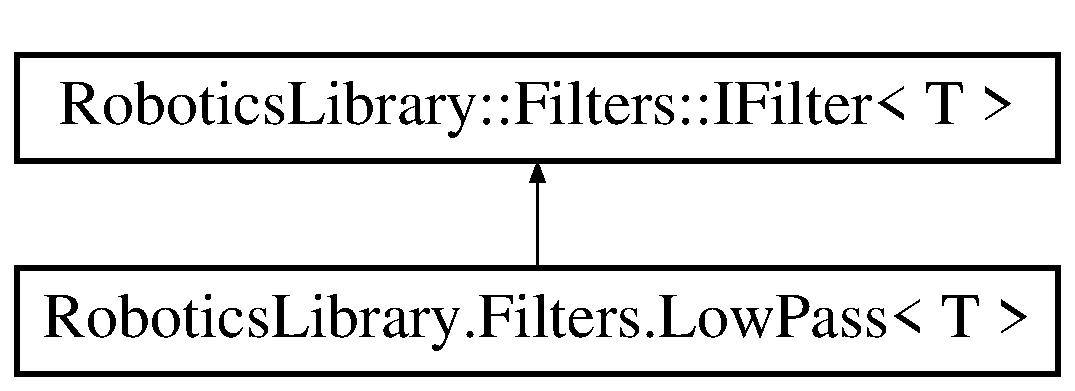
\includegraphics[height=2.000000cm]{d4/d3a/class_robotics_library_1_1_filters_1_1_low_pass}
\end{center}
\end{figure}
\subsection*{Public Member Functions}
\begin{DoxyCompactItemize}
\item 
\hyperlink{class_robotics_library_1_1_filters_1_1_low_pass_ada79534600a7f4a4dab17c40976a2f74}{Low\+Pass} (double \hyperlink{class_robotics_library_1_1_filters_1_1_low_pass_aa10538fde21bb3d7a4c5640b615c4013}{L\+P\+Fk}=0.\+25)
\begin{DoxyCompactList}\small\item\em Constructs a low pass filter with time constant {\ttfamily L\+P\+Fk}.\end{DoxyCompactList}\item 
void \hyperlink{class_robotics_library_1_1_filters_1_1_low_pass_adba4c542b4935845404729ebb2222b72}{Feed} (T Input)
\begin{DoxyCompactList}\small\item\em Feeds a value into the filter. \end{DoxyCompactList}\item 
void \hyperlink{class_robotics_library_1_1_filters_1_1_low_pass_a9b8d610c0f54a17e84ea5e9252c9e215}{Feed} (T Input, T Rate)
\begin{DoxyCompactList}\small\item\em Feeds filter with specified rate. Not used for average filter. \end{DoxyCompactList}\item 
void \hyperlink{class_robotics_library_1_1_filters_1_1_low_pass_a4cc6f562359e222b75c634075cfc4881}{Reset} ()
\begin{DoxyCompactList}\small\item\em Resets the low pass filter to the default value of {\ttfamily T} \end{DoxyCompactList}\end{DoxyCompactItemize}
\subsection*{Properties}
\begin{DoxyCompactItemize}
\item 
T \hyperlink{class_robotics_library_1_1_filters_1_1_low_pass_a83f66e4bfd6737c56614f3bb9a73876f}{Output}\hspace{0.3cm}{\ttfamily  \mbox{[}get, private set\mbox{]}}
\item 
double \hyperlink{class_robotics_library_1_1_filters_1_1_low_pass_aa10538fde21bb3d7a4c5640b615c4013}{L\+P\+Fk}\hspace{0.3cm}{\ttfamily  \mbox{[}get, private set\mbox{]}}
\end{DoxyCompactItemize}
\subsection*{Private Attributes}
\begin{DoxyCompactItemize}
\item 
T \hyperlink{class_robotics_library_1_1_filters_1_1_low_pass_a0d00e590f0cdafdd06200870121e9b07}{Last\+Value}
\end{DoxyCompactItemize}


\subsection{Detailed Description}
The Low Pass filter is intended for use as an average-\/gathering system, using a low pass filter with time constant {\ttfamily L\+P\+Fk}.

Implementation Details\+:

$\ast$\+Construct Low Pass filter given a time constant {\ttfamily L\+P\+Fk}

$\ast$\+Iteratively add values into the filter using {\ttfamily \hyperlink{class_robotics_library_1_1_filters_1_1_low_pass_adba4c542b4935845404729ebb2222b72}{Feed(\+T Input)}}

$\ast$\+Get the filter output by calling {\ttfamily Your\+Filter\+Instance.\+Output}


\begin{DoxyTemplParams}{Template Parameters}
{\em T} & A type, which must be a numeric.\\
\hline
\end{DoxyTemplParams}
\begin{Desc}
\item[Type Constraints]\begin{description}
\item[{\em T} : {\em I\+Comparable}]\end{description}
\end{Desc}


\subsection{Constructor \& Destructor Documentation}
\mbox{\Hypertarget{class_robotics_library_1_1_filters_1_1_low_pass_ada79534600a7f4a4dab17c40976a2f74}\label{class_robotics_library_1_1_filters_1_1_low_pass_ada79534600a7f4a4dab17c40976a2f74}} 
\index{Robotics\+Library\+::\+Filters\+::\+Low\+Pass@{Robotics\+Library\+::\+Filters\+::\+Low\+Pass}!Low\+Pass@{Low\+Pass}}
\index{Low\+Pass@{Low\+Pass}!Robotics\+Library\+::\+Filters\+::\+Low\+Pass@{Robotics\+Library\+::\+Filters\+::\+Low\+Pass}}
\subsubsection{\texorpdfstring{Low\+Pass()}{LowPass()}}
{\footnotesize\ttfamily \hyperlink{class_robotics_library_1_1_filters_1_1_low_pass}{Robotics\+Library.\+Filters.\+Low\+Pass}$<$ T $>$.\hyperlink{class_robotics_library_1_1_filters_1_1_low_pass}{Low\+Pass} (\begin{DoxyParamCaption}\item[{double}]{L\+P\+Fk = {\ttfamily 0.25} }\end{DoxyParamCaption})}



Constructs a low pass filter with time constant {\ttfamily L\+P\+Fk}.


\begin{DoxyParams}{Parameters}
{\em L\+P\+Fk} & Low Pass Filter Time Constant.\\
\hline
\end{DoxyParams}


\subsection{Member Function Documentation}
\mbox{\Hypertarget{class_robotics_library_1_1_filters_1_1_low_pass_adba4c542b4935845404729ebb2222b72}\label{class_robotics_library_1_1_filters_1_1_low_pass_adba4c542b4935845404729ebb2222b72}} 
\index{Robotics\+Library\+::\+Filters\+::\+Low\+Pass@{Robotics\+Library\+::\+Filters\+::\+Low\+Pass}!Feed@{Feed}}
\index{Feed@{Feed}!Robotics\+Library\+::\+Filters\+::\+Low\+Pass@{Robotics\+Library\+::\+Filters\+::\+Low\+Pass}}
\subsubsection{\texorpdfstring{Feed()}{Feed()}\hspace{0.1cm}{\footnotesize\ttfamily [1/2]}}
{\footnotesize\ttfamily void \hyperlink{class_robotics_library_1_1_filters_1_1_low_pass}{Robotics\+Library.\+Filters.\+Low\+Pass}$<$ T $>$.Feed (\begin{DoxyParamCaption}\item[{T}]{Input }\end{DoxyParamCaption})}



Feeds a value into the filter. 


\begin{DoxyParams}{Parameters}
{\em Input} & Value to feed into the filter.\\
\hline
\end{DoxyParams}


Implements \hyperlink{interface_robotics_library_1_1_filters_1_1_i_filter_a64855020add7b0354c2773696521c84e}{Robotics\+Library.\+Filters.\+I\+Filter$<$ T $>$}.

\mbox{\Hypertarget{class_robotics_library_1_1_filters_1_1_low_pass_a9b8d610c0f54a17e84ea5e9252c9e215}\label{class_robotics_library_1_1_filters_1_1_low_pass_a9b8d610c0f54a17e84ea5e9252c9e215}} 
\index{Robotics\+Library\+::\+Filters\+::\+Low\+Pass@{Robotics\+Library\+::\+Filters\+::\+Low\+Pass}!Feed@{Feed}}
\index{Feed@{Feed}!Robotics\+Library\+::\+Filters\+::\+Low\+Pass@{Robotics\+Library\+::\+Filters\+::\+Low\+Pass}}
\subsubsection{\texorpdfstring{Feed()}{Feed()}\hspace{0.1cm}{\footnotesize\ttfamily [2/2]}}
{\footnotesize\ttfamily void \hyperlink{class_robotics_library_1_1_filters_1_1_low_pass}{Robotics\+Library.\+Filters.\+Low\+Pass}$<$ T $>$.Feed (\begin{DoxyParamCaption}\item[{T}]{Input,  }\item[{T}]{Rate }\end{DoxyParamCaption})}



Feeds filter with specified rate. Not used for average filter. 


\begin{DoxyParams}{Parameters}
{\em Input} & Value to feed into the filer.\\
\hline
{\em Rate} & Current rate to feed into the filter.\\
\hline
\end{DoxyParams}


Implements \hyperlink{interface_robotics_library_1_1_filters_1_1_i_filter_a24d363fb2957923a256448e04634d9ca}{Robotics\+Library.\+Filters.\+I\+Filter$<$ T $>$}.

\mbox{\Hypertarget{class_robotics_library_1_1_filters_1_1_low_pass_a4cc6f562359e222b75c634075cfc4881}\label{class_robotics_library_1_1_filters_1_1_low_pass_a4cc6f562359e222b75c634075cfc4881}} 
\index{Robotics\+Library\+::\+Filters\+::\+Low\+Pass@{Robotics\+Library\+::\+Filters\+::\+Low\+Pass}!Reset@{Reset}}
\index{Reset@{Reset}!Robotics\+Library\+::\+Filters\+::\+Low\+Pass@{Robotics\+Library\+::\+Filters\+::\+Low\+Pass}}
\subsubsection{\texorpdfstring{Reset()}{Reset()}}
{\footnotesize\ttfamily void \hyperlink{class_robotics_library_1_1_filters_1_1_low_pass}{Robotics\+Library.\+Filters.\+Low\+Pass}$<$ T $>$.Reset (\begin{DoxyParamCaption}{ }\end{DoxyParamCaption})}



Resets the low pass filter to the default value of {\ttfamily T} 



\subsection{Member Data Documentation}
\mbox{\Hypertarget{class_robotics_library_1_1_filters_1_1_low_pass_a0d00e590f0cdafdd06200870121e9b07}\label{class_robotics_library_1_1_filters_1_1_low_pass_a0d00e590f0cdafdd06200870121e9b07}} 
\index{Robotics\+Library\+::\+Filters\+::\+Low\+Pass@{Robotics\+Library\+::\+Filters\+::\+Low\+Pass}!Last\+Value@{Last\+Value}}
\index{Last\+Value@{Last\+Value}!Robotics\+Library\+::\+Filters\+::\+Low\+Pass@{Robotics\+Library\+::\+Filters\+::\+Low\+Pass}}
\subsubsection{\texorpdfstring{Last\+Value}{LastValue}}
{\footnotesize\ttfamily T \hyperlink{class_robotics_library_1_1_filters_1_1_low_pass}{Robotics\+Library.\+Filters.\+Low\+Pass}$<$ T $>$.Last\+Value\hspace{0.3cm}{\ttfamily [private]}}



\subsection{Property Documentation}
\mbox{\Hypertarget{class_robotics_library_1_1_filters_1_1_low_pass_aa10538fde21bb3d7a4c5640b615c4013}\label{class_robotics_library_1_1_filters_1_1_low_pass_aa10538fde21bb3d7a4c5640b615c4013}} 
\index{Robotics\+Library\+::\+Filters\+::\+Low\+Pass@{Robotics\+Library\+::\+Filters\+::\+Low\+Pass}!L\+P\+Fk@{L\+P\+Fk}}
\index{L\+P\+Fk@{L\+P\+Fk}!Robotics\+Library\+::\+Filters\+::\+Low\+Pass@{Robotics\+Library\+::\+Filters\+::\+Low\+Pass}}
\subsubsection{\texorpdfstring{L\+P\+Fk}{LPFk}}
{\footnotesize\ttfamily double \hyperlink{class_robotics_library_1_1_filters_1_1_low_pass}{Robotics\+Library.\+Filters.\+Low\+Pass}$<$ T $>$.L\+P\+Fk\hspace{0.3cm}{\ttfamily [get]}, {\ttfamily [private set]}}

\mbox{\Hypertarget{class_robotics_library_1_1_filters_1_1_low_pass_a83f66e4bfd6737c56614f3bb9a73876f}\label{class_robotics_library_1_1_filters_1_1_low_pass_a83f66e4bfd6737c56614f3bb9a73876f}} 
\index{Robotics\+Library\+::\+Filters\+::\+Low\+Pass@{Robotics\+Library\+::\+Filters\+::\+Low\+Pass}!Output@{Output}}
\index{Output@{Output}!Robotics\+Library\+::\+Filters\+::\+Low\+Pass@{Robotics\+Library\+::\+Filters\+::\+Low\+Pass}}
\subsubsection{\texorpdfstring{Output}{Output}}
{\footnotesize\ttfamily T \hyperlink{class_robotics_library_1_1_filters_1_1_low_pass}{Robotics\+Library.\+Filters.\+Low\+Pass}$<$ T $>$.Output\hspace{0.3cm}{\ttfamily [get]}, {\ttfamily [private set]}}



The documentation for this class was generated from the following file\+:\begin{DoxyCompactItemize}
\item 
C\+:/\+Users/jaden/\+Documents/\+Git\+Hub/2017-\/18/science/\+Science Library/\+Filters/\hyperlink{_low_pass_8cs}{Low\+Pass.\+cs}\end{DoxyCompactItemize}

\hypertarget{class_robotics_library_1_1_communications_1_1_message}{}\section{Robotics\+Library.\+Communications.\+Message Class Reference}
\label{class_robotics_library_1_1_communications_1_1_message}\index{Robotics\+Library.\+Communications.\+Message@{Robotics\+Library.\+Communications.\+Message}}


This class is intended to encode incoming data.  


\subsection*{Public Member Functions}
\begin{DoxyCompactItemize}
\item 
\hyperlink{class_robotics_library_1_1_communications_1_1_message_a9e6e25188a64e3cc1c71282c2578cc4e}{Message} (byte\mbox{[}$\,$\mbox{]} Incoming\+Data, I\+P\+End\+Point \hyperlink{class_robotics_library_1_1_communications_1_1_message_a51a162a1d00eb020c5af595cc84bf604}{From})
\begin{DoxyCompactList}\small\item\em Constructs a message given incoming data. Data encoded with\+: Timestamp data\mbox{[}0\mbox{]} to data\mbox{[}3\mbox{]} ID at data\mbox{[}4\mbox{]} Data encoded after data\mbox{[}4\mbox{]}, i.\+e. data\mbox{[}5\+:\mbox{]} \end{DoxyCompactList}\end{DoxyCompactItemize}
\subsection*{Public Attributes}
\begin{DoxyCompactItemize}
\item 
int \hyperlink{class_robotics_library_1_1_communications_1_1_message_ae1ab1ac8b229f8ba8bc9ff8762c83236}{Timesamp}
\item 
byte \mbox{[}$\,$\mbox{]} \hyperlink{class_robotics_library_1_1_communications_1_1_message_a69bb31eb51f778726ae40b2257e7e053}{Data}
\item 
I\+P\+End\+Point \hyperlink{class_robotics_library_1_1_communications_1_1_message_a51a162a1d00eb020c5af595cc84bf604}{From}
\end{DoxyCompactItemize}


\subsection{Detailed Description}
This class is intended to encode incoming data. 



\subsection{Constructor \& Destructor Documentation}
\mbox{\Hypertarget{class_robotics_library_1_1_communications_1_1_message_a9e6e25188a64e3cc1c71282c2578cc4e}\label{class_robotics_library_1_1_communications_1_1_message_a9e6e25188a64e3cc1c71282c2578cc4e}} 
\index{Robotics\+Library\+::\+Communications\+::\+Message@{Robotics\+Library\+::\+Communications\+::\+Message}!Message@{Message}}
\index{Message@{Message}!Robotics\+Library\+::\+Communications\+::\+Message@{Robotics\+Library\+::\+Communications\+::\+Message}}
\subsubsection{\texorpdfstring{Message()}{Message()}}
{\footnotesize\ttfamily Robotics\+Library.\+Communications.\+Message.\+Message (\begin{DoxyParamCaption}\item[{byte \mbox{[}$\,$\mbox{]}}]{Incoming\+Data,  }\item[{I\+P\+End\+Point}]{From }\end{DoxyParamCaption})}



Constructs a message given incoming data. Data encoded with\+: Timestamp data\mbox{[}0\mbox{]} to data\mbox{[}3\mbox{]} ID at data\mbox{[}4\mbox{]} Data encoded after data\mbox{[}4\mbox{]}, i.\+e. data\mbox{[}5\+:\mbox{]} 


\begin{DoxyParams}{Parameters}
{\em Incoming\+Data} & Incoming data array\\
\hline
{\em From} & Given from endpoint\\
\hline
\end{DoxyParams}


\subsection{Member Data Documentation}
\mbox{\Hypertarget{class_robotics_library_1_1_communications_1_1_message_a69bb31eb51f778726ae40b2257e7e053}\label{class_robotics_library_1_1_communications_1_1_message_a69bb31eb51f778726ae40b2257e7e053}} 
\index{Robotics\+Library\+::\+Communications\+::\+Message@{Robotics\+Library\+::\+Communications\+::\+Message}!Data@{Data}}
\index{Data@{Data}!Robotics\+Library\+::\+Communications\+::\+Message@{Robotics\+Library\+::\+Communications\+::\+Message}}
\subsubsection{\texorpdfstring{Data}{Data}}
{\footnotesize\ttfamily byte \mbox{[}$\,$\mbox{]} Robotics\+Library.\+Communications.\+Message.\+Data}

\mbox{\Hypertarget{class_robotics_library_1_1_communications_1_1_message_a51a162a1d00eb020c5af595cc84bf604}\label{class_robotics_library_1_1_communications_1_1_message_a51a162a1d00eb020c5af595cc84bf604}} 
\index{Robotics\+Library\+::\+Communications\+::\+Message@{Robotics\+Library\+::\+Communications\+::\+Message}!From@{From}}
\index{From@{From}!Robotics\+Library\+::\+Communications\+::\+Message@{Robotics\+Library\+::\+Communications\+::\+Message}}
\subsubsection{\texorpdfstring{From}{From}}
{\footnotesize\ttfamily I\+P\+End\+Point Robotics\+Library.\+Communications.\+Message.\+From}

\mbox{\Hypertarget{class_robotics_library_1_1_communications_1_1_message_ae1ab1ac8b229f8ba8bc9ff8762c83236}\label{class_robotics_library_1_1_communications_1_1_message_ae1ab1ac8b229f8ba8bc9ff8762c83236}} 
\index{Robotics\+Library\+::\+Communications\+::\+Message@{Robotics\+Library\+::\+Communications\+::\+Message}!Timesamp@{Timesamp}}
\index{Timesamp@{Timesamp}!Robotics\+Library\+::\+Communications\+::\+Message@{Robotics\+Library\+::\+Communications\+::\+Message}}
\subsubsection{\texorpdfstring{Timesamp}{Timesamp}}
{\footnotesize\ttfamily int Robotics\+Library.\+Communications.\+Message.\+Timesamp}



The documentation for this class was generated from the following file\+:\begin{DoxyCompactItemize}
\item 
Communications/\hyperlink{_message_8cs}{Message.\+cs}\end{DoxyCompactItemize}

\hypertarget{class_robotics_library_1_1_communications_1_1_packet}{}\section{Robotics\+Library.\+Communications.\+Packet Class Reference}
\label{class_robotics_library_1_1_communications_1_1_packet}\index{Robotics\+Library.\+Communications.\+Packet@{Robotics\+Library.\+Communications.\+Packet}}


Handles packet architecture.  


\subsection*{Public Member Functions}
\begin{DoxyCompactItemize}
\item 
\hyperlink{class_robotics_library_1_1_communications_1_1_packet_a959df60d7fb5b840f1ac17f2558287d9}{Packet} (int \hyperlink{class_robotics_library_1_1_communications_1_1_packet_a6ed48c10bbd9b06fcb2dbd8172106728}{Id}, I\+P\+End\+Point \hyperlink{class_robotics_library_1_1_communications_1_1_packet_a394c86b3647f472f3a24837bba067338}{Packet\+Endpoint}=null)
\begin{DoxyCompactList}\small\item\em Constructs new packet of given ID. \end{DoxyCompactList}\item 
void \hyperlink{class_robotics_library_1_1_communications_1_1_packet_a047afd1596cdeb703ff7fe965a6a15ee}{Append\+Data} (byte\mbox{[}$\,$\mbox{]} \hyperlink{class_robotics_library_1_1_communications_1_1_packet_a16cae05afc6eda9dad5592095528d19a}{Data})
\begin{DoxyCompactList}\small\item\em Appends data to packet. \end{DoxyCompactList}\item 
bool \hyperlink{class_robotics_library_1_1_communications_1_1_packet_aea2ef8cc2357083a18bf3c1da0b0bdec}{Send} ()
\begin{DoxyCompactList}\small\item\em Sends packet \end{DoxyCompactList}\end{DoxyCompactItemize}
\subsection*{Static Public Member Functions}
\begin{DoxyCompactItemize}
\item 
static void \hyperlink{class_robotics_library_1_1_communications_1_1_packet_a95a0bb161aa290379b3d016b02707e93}{Set\+Default\+Endpoint} (I\+P\+End\+Point Endpoint)
\begin{DoxyCompactList}\small\item\em Sets the packet class\textquotesingle{}s default Endpoint. \end{DoxyCompactList}\end{DoxyCompactItemize}
\subsection*{Private Member Functions}
\begin{DoxyCompactItemize}
\item 
void \hyperlink{class_robotics_library_1_1_communications_1_1_packet_a7003488a8d9d08f24a11953fdec60960}{Set\+Time} ()
\begin{DoxyCompactList}\small\item\em Sets time for packet. Internal use only. \end{DoxyCompactList}\end{DoxyCompactItemize}
\subsection*{Private Attributes}
\begin{DoxyCompactItemize}
\item 
byte \hyperlink{class_robotics_library_1_1_communications_1_1_packet_a6ed48c10bbd9b06fcb2dbd8172106728}{Id}
\item 
byte \mbox{[}$\,$\mbox{]} \hyperlink{class_robotics_library_1_1_communications_1_1_packet_aeaf9b3ec1923f1126c2025b1dd909468}{Timestamp}
\item 
byte \mbox{[}$\,$\mbox{]} \hyperlink{class_robotics_library_1_1_communications_1_1_packet_a16cae05afc6eda9dad5592095528d19a}{Data}
\item 
I\+P\+End\+Point \hyperlink{class_robotics_library_1_1_communications_1_1_packet_a394c86b3647f472f3a24837bba067338}{Packet\+Endpoint}
\item 
Tcp\+Client \hyperlink{class_robotics_library_1_1_communications_1_1_packet_ab276ef9ce5f4ae88a1e3e0d70a40a1f2}{Client}
\end{DoxyCompactItemize}
\subsection*{Static Private Attributes}
\begin{DoxyCompactItemize}
\item 
static I\+P\+End\+Point \hyperlink{class_robotics_library_1_1_communications_1_1_packet_ac7aa1b8ff94b4e190b284ac7b8ac4b4a}{Default\+Endpoint} = new I\+P\+End\+Point(I\+P\+Address.\+Parse(\char`\"{}192.\+168.\+0.\+1\char`\"{}), 600)
\end{DoxyCompactItemize}


\subsection{Detailed Description}
Handles packet architecture. 



\subsection{Constructor \& Destructor Documentation}
\mbox{\Hypertarget{class_robotics_library_1_1_communications_1_1_packet_a959df60d7fb5b840f1ac17f2558287d9}\label{class_robotics_library_1_1_communications_1_1_packet_a959df60d7fb5b840f1ac17f2558287d9}} 
\index{Robotics\+Library\+::\+Communications\+::\+Packet@{Robotics\+Library\+::\+Communications\+::\+Packet}!Packet@{Packet}}
\index{Packet@{Packet}!Robotics\+Library\+::\+Communications\+::\+Packet@{Robotics\+Library\+::\+Communications\+::\+Packet}}
\subsubsection{\texorpdfstring{Packet()}{Packet()}}
{\footnotesize\ttfamily Robotics\+Library.\+Communications.\+Packet.\+Packet (\begin{DoxyParamCaption}\item[{int}]{Id,  }\item[{I\+P\+End\+Point}]{Packet\+Endpoint = {\ttfamily null} }\end{DoxyParamCaption})}



Constructs new packet of given ID. 


\begin{DoxyParams}{Parameters}
{\em Id} & \\
\hline
{\em Packet\+Endpoint} & Endpoint for the packet. If null, defaults to given {\ttfamily Default\+Endpoint}\\
\hline
\end{DoxyParams}


\subsection{Member Function Documentation}
\mbox{\Hypertarget{class_robotics_library_1_1_communications_1_1_packet_a047afd1596cdeb703ff7fe965a6a15ee}\label{class_robotics_library_1_1_communications_1_1_packet_a047afd1596cdeb703ff7fe965a6a15ee}} 
\index{Robotics\+Library\+::\+Communications\+::\+Packet@{Robotics\+Library\+::\+Communications\+::\+Packet}!Append\+Data@{Append\+Data}}
\index{Append\+Data@{Append\+Data}!Robotics\+Library\+::\+Communications\+::\+Packet@{Robotics\+Library\+::\+Communications\+::\+Packet}}
\subsubsection{\texorpdfstring{Append\+Data()}{AppendData()}}
{\footnotesize\ttfamily void Robotics\+Library.\+Communications.\+Packet.\+Append\+Data (\begin{DoxyParamCaption}\item[{byte \mbox{[}$\,$\mbox{]}}]{Data }\end{DoxyParamCaption})}



Appends data to packet. 


\begin{DoxyParams}{Parameters}
{\em Data} & Data to append to packet.\\
\hline
\end{DoxyParams}
\mbox{\Hypertarget{class_robotics_library_1_1_communications_1_1_packet_aea2ef8cc2357083a18bf3c1da0b0bdec}\label{class_robotics_library_1_1_communications_1_1_packet_aea2ef8cc2357083a18bf3c1da0b0bdec}} 
\index{Robotics\+Library\+::\+Communications\+::\+Packet@{Robotics\+Library\+::\+Communications\+::\+Packet}!Send@{Send}}
\index{Send@{Send}!Robotics\+Library\+::\+Communications\+::\+Packet@{Robotics\+Library\+::\+Communications\+::\+Packet}}
\subsubsection{\texorpdfstring{Send()}{Send()}}
{\footnotesize\ttfamily bool Robotics\+Library.\+Communications.\+Packet.\+Send (\begin{DoxyParamCaption}{ }\end{DoxyParamCaption})}



Sends packet 

\begin{DoxyReturn}{Returns}
true if Send successful, false is Send unsuccessful. 
\end{DoxyReturn}
\mbox{\Hypertarget{class_robotics_library_1_1_communications_1_1_packet_a95a0bb161aa290379b3d016b02707e93}\label{class_robotics_library_1_1_communications_1_1_packet_a95a0bb161aa290379b3d016b02707e93}} 
\index{Robotics\+Library\+::\+Communications\+::\+Packet@{Robotics\+Library\+::\+Communications\+::\+Packet}!Set\+Default\+Endpoint@{Set\+Default\+Endpoint}}
\index{Set\+Default\+Endpoint@{Set\+Default\+Endpoint}!Robotics\+Library\+::\+Communications\+::\+Packet@{Robotics\+Library\+::\+Communications\+::\+Packet}}
\subsubsection{\texorpdfstring{Set\+Default\+Endpoint()}{SetDefaultEndpoint()}}
{\footnotesize\ttfamily static void Robotics\+Library.\+Communications.\+Packet.\+Set\+Default\+Endpoint (\begin{DoxyParamCaption}\item[{I\+P\+End\+Point}]{Endpoint }\end{DoxyParamCaption})\hspace{0.3cm}{\ttfamily [static]}}



Sets the packet class\textquotesingle{}s default Endpoint. 


\begin{DoxyParams}{Parameters}
{\em Endpoint} & New default endpoint for the packet class. \\
\hline
\end{DoxyParams}
\mbox{\Hypertarget{class_robotics_library_1_1_communications_1_1_packet_a7003488a8d9d08f24a11953fdec60960}\label{class_robotics_library_1_1_communications_1_1_packet_a7003488a8d9d08f24a11953fdec60960}} 
\index{Robotics\+Library\+::\+Communications\+::\+Packet@{Robotics\+Library\+::\+Communications\+::\+Packet}!Set\+Time@{Set\+Time}}
\index{Set\+Time@{Set\+Time}!Robotics\+Library\+::\+Communications\+::\+Packet@{Robotics\+Library\+::\+Communications\+::\+Packet}}
\subsubsection{\texorpdfstring{Set\+Time()}{SetTime()}}
{\footnotesize\ttfamily void Robotics\+Library.\+Communications.\+Packet.\+Set\+Time (\begin{DoxyParamCaption}{ }\end{DoxyParamCaption})\hspace{0.3cm}{\ttfamily [private]}}



Sets time for packet. Internal use only. 



\subsection{Member Data Documentation}
\mbox{\Hypertarget{class_robotics_library_1_1_communications_1_1_packet_ab276ef9ce5f4ae88a1e3e0d70a40a1f2}\label{class_robotics_library_1_1_communications_1_1_packet_ab276ef9ce5f4ae88a1e3e0d70a40a1f2}} 
\index{Robotics\+Library\+::\+Communications\+::\+Packet@{Robotics\+Library\+::\+Communications\+::\+Packet}!Client@{Client}}
\index{Client@{Client}!Robotics\+Library\+::\+Communications\+::\+Packet@{Robotics\+Library\+::\+Communications\+::\+Packet}}
\subsubsection{\texorpdfstring{Client}{Client}}
{\footnotesize\ttfamily Tcp\+Client Robotics\+Library.\+Communications.\+Packet.\+Client\hspace{0.3cm}{\ttfamily [private]}}

\mbox{\Hypertarget{class_robotics_library_1_1_communications_1_1_packet_a16cae05afc6eda9dad5592095528d19a}\label{class_robotics_library_1_1_communications_1_1_packet_a16cae05afc6eda9dad5592095528d19a}} 
\index{Robotics\+Library\+::\+Communications\+::\+Packet@{Robotics\+Library\+::\+Communications\+::\+Packet}!Data@{Data}}
\index{Data@{Data}!Robotics\+Library\+::\+Communications\+::\+Packet@{Robotics\+Library\+::\+Communications\+::\+Packet}}
\subsubsection{\texorpdfstring{Data}{Data}}
{\footnotesize\ttfamily byte \mbox{[}$\,$\mbox{]} Robotics\+Library.\+Communications.\+Packet.\+Data\hspace{0.3cm}{\ttfamily [private]}}

\mbox{\Hypertarget{class_robotics_library_1_1_communications_1_1_packet_ac7aa1b8ff94b4e190b284ac7b8ac4b4a}\label{class_robotics_library_1_1_communications_1_1_packet_ac7aa1b8ff94b4e190b284ac7b8ac4b4a}} 
\index{Robotics\+Library\+::\+Communications\+::\+Packet@{Robotics\+Library\+::\+Communications\+::\+Packet}!Default\+Endpoint@{Default\+Endpoint}}
\index{Default\+Endpoint@{Default\+Endpoint}!Robotics\+Library\+::\+Communications\+::\+Packet@{Robotics\+Library\+::\+Communications\+::\+Packet}}
\subsubsection{\texorpdfstring{Default\+Endpoint}{DefaultEndpoint}}
{\footnotesize\ttfamily I\+P\+End\+Point Robotics\+Library.\+Communications.\+Packet.\+Default\+Endpoint = new I\+P\+End\+Point(I\+P\+Address.\+Parse(\char`\"{}192.\+168.\+0.\+1\char`\"{}), 600)\hspace{0.3cm}{\ttfamily [static]}, {\ttfamily [private]}}

\mbox{\Hypertarget{class_robotics_library_1_1_communications_1_1_packet_a6ed48c10bbd9b06fcb2dbd8172106728}\label{class_robotics_library_1_1_communications_1_1_packet_a6ed48c10bbd9b06fcb2dbd8172106728}} 
\index{Robotics\+Library\+::\+Communications\+::\+Packet@{Robotics\+Library\+::\+Communications\+::\+Packet}!Id@{Id}}
\index{Id@{Id}!Robotics\+Library\+::\+Communications\+::\+Packet@{Robotics\+Library\+::\+Communications\+::\+Packet}}
\subsubsection{\texorpdfstring{Id}{Id}}
{\footnotesize\ttfamily byte Robotics\+Library.\+Communications.\+Packet.\+Id\hspace{0.3cm}{\ttfamily [private]}}

\mbox{\Hypertarget{class_robotics_library_1_1_communications_1_1_packet_a394c86b3647f472f3a24837bba067338}\label{class_robotics_library_1_1_communications_1_1_packet_a394c86b3647f472f3a24837bba067338}} 
\index{Robotics\+Library\+::\+Communications\+::\+Packet@{Robotics\+Library\+::\+Communications\+::\+Packet}!Packet\+Endpoint@{Packet\+Endpoint}}
\index{Packet\+Endpoint@{Packet\+Endpoint}!Robotics\+Library\+::\+Communications\+::\+Packet@{Robotics\+Library\+::\+Communications\+::\+Packet}}
\subsubsection{\texorpdfstring{Packet\+Endpoint}{PacketEndpoint}}
{\footnotesize\ttfamily I\+P\+End\+Point Robotics\+Library.\+Communications.\+Packet.\+Packet\+Endpoint\hspace{0.3cm}{\ttfamily [private]}}

\mbox{\Hypertarget{class_robotics_library_1_1_communications_1_1_packet_aeaf9b3ec1923f1126c2025b1dd909468}\label{class_robotics_library_1_1_communications_1_1_packet_aeaf9b3ec1923f1126c2025b1dd909468}} 
\index{Robotics\+Library\+::\+Communications\+::\+Packet@{Robotics\+Library\+::\+Communications\+::\+Packet}!Timestamp@{Timestamp}}
\index{Timestamp@{Timestamp}!Robotics\+Library\+::\+Communications\+::\+Packet@{Robotics\+Library\+::\+Communications\+::\+Packet}}
\subsubsection{\texorpdfstring{Timestamp}{Timestamp}}
{\footnotesize\ttfamily byte \mbox{[}$\,$\mbox{]} Robotics\+Library.\+Communications.\+Packet.\+Timestamp\hspace{0.3cm}{\ttfamily [private]}}



The documentation for this class was generated from the following file\+:\begin{DoxyCompactItemize}
\item 
C\+:/\+Users/jaden/\+Documents/\+Git\+Hub/2017-\/18/science/\+Science Library/\+Communications/\hyperlink{_packet_8cs}{Packet.\+cs}\end{DoxyCompactItemize}

\hypertarget{class_robotics_library_1_1_communications_1_1_parse}{}\section{Robotics\+Library.\+Communications.\+Parse Class Reference}
\label{class_robotics_library_1_1_communications_1_1_parse}\index{Robotics\+Library.\+Communications.\+Parse@{Robotics\+Library.\+Communications.\+Parse}}


Handles packet parsing, using handlers of incoming message I\+Ds.  


\subsection*{Public Member Functions}
\begin{DoxyCompactItemize}
\item 
delegate void \hyperlink{class_robotics_library_1_1_communications_1_1_parse_a592095b5638ced6eacabbce7acdb5e75}{Parse\+Method} (\hyperlink{class_robotics_library_1_1_communications_1_1_message}{Message} New\+Message)
\end{DoxyCompactItemize}
\subsection*{Static Public Member Functions}
\begin{DoxyCompactItemize}
\item 
static void \hyperlink{class_robotics_library_1_1_communications_1_1_parse_a2edbe1773ccbf303fb505ce0ad2ee838}{Set\+Parse\+Handler} (byte Message\+Id, \hyperlink{class_robotics_library_1_1_communications_1_1_parse_a592095b5638ced6eacabbce7acdb5e75}{Parse\+Method} \hyperlink{class_robotics_library_1_1_communications_1_1_parse_a592095b5638ced6eacabbce7acdb5e75}{Parse\+Method})
\begin{DoxyCompactList}\small\item\em Sets the handler for parsing of the appropriate Message\+Id. \end{DoxyCompactList}\item 
static void \hyperlink{class_robotics_library_1_1_communications_1_1_parse_ad148efeadd6ab19f2fa53d4b90acf890}{Parse\+Message} (\hyperlink{class_robotics_library_1_1_communications_1_1_message}{Message} New\+Message)
\begin{DoxyCompactList}\small\item\em Appropriately parses incoming message. \end{DoxyCompactList}\end{DoxyCompactItemize}
\subsection*{Static Private Attributes}
\begin{DoxyCompactItemize}
\item 
static \hyperlink{class_robotics_library_1_1_communications_1_1_parse_a592095b5638ced6eacabbce7acdb5e75}{Parse\+Method} \mbox{[}$\,$\mbox{]} \hyperlink{class_robotics_library_1_1_communications_1_1_parse_aa2e45508e6d9222047bfbec487628c87}{Parsing\+Handlers} = new \hyperlink{class_robotics_library_1_1_communications_1_1_parse_a592095b5638ced6eacabbce7acdb5e75}{Parse\+Method}\mbox{[}256\mbox{]}
\end{DoxyCompactItemize}


\subsection{Detailed Description}
Handles packet parsing, using handlers of incoming message I\+Ds. 



\subsection{Member Function Documentation}
\mbox{\Hypertarget{class_robotics_library_1_1_communications_1_1_parse_ad148efeadd6ab19f2fa53d4b90acf890}\label{class_robotics_library_1_1_communications_1_1_parse_ad148efeadd6ab19f2fa53d4b90acf890}} 
\index{Robotics\+Library\+::\+Communications\+::\+Parse@{Robotics\+Library\+::\+Communications\+::\+Parse}!Parse\+Message@{Parse\+Message}}
\index{Parse\+Message@{Parse\+Message}!Robotics\+Library\+::\+Communications\+::\+Parse@{Robotics\+Library\+::\+Communications\+::\+Parse}}
\subsubsection{\texorpdfstring{Parse\+Message()}{ParseMessage()}}
{\footnotesize\ttfamily static void Robotics\+Library.\+Communications.\+Parse.\+Parse\+Message (\begin{DoxyParamCaption}\item[{\hyperlink{class_robotics_library_1_1_communications_1_1_message}{Message}}]{New\+Message }\end{DoxyParamCaption})\hspace{0.3cm}{\ttfamily [static]}}



Appropriately parses incoming message. 


\begin{DoxyParams}{Parameters}
{\em New\+Message} & \hyperlink{class_robotics_library_1_1_communications_1_1_message}{Message} to parse.\\
\hline
\end{DoxyParams}
\mbox{\Hypertarget{class_robotics_library_1_1_communications_1_1_parse_a592095b5638ced6eacabbce7acdb5e75}\label{class_robotics_library_1_1_communications_1_1_parse_a592095b5638ced6eacabbce7acdb5e75}} 
\index{Robotics\+Library\+::\+Communications\+::\+Parse@{Robotics\+Library\+::\+Communications\+::\+Parse}!Parse\+Method@{Parse\+Method}}
\index{Parse\+Method@{Parse\+Method}!Robotics\+Library\+::\+Communications\+::\+Parse@{Robotics\+Library\+::\+Communications\+::\+Parse}}
\subsubsection{\texorpdfstring{Parse\+Method()}{ParseMethod()}}
{\footnotesize\ttfamily delegate void Robotics\+Library.\+Communications.\+Parse.\+Parse\+Method (\begin{DoxyParamCaption}\item[{\hyperlink{class_robotics_library_1_1_communications_1_1_message}{Message}}]{New\+Message }\end{DoxyParamCaption})}

\mbox{\Hypertarget{class_robotics_library_1_1_communications_1_1_parse_a2edbe1773ccbf303fb505ce0ad2ee838}\label{class_robotics_library_1_1_communications_1_1_parse_a2edbe1773ccbf303fb505ce0ad2ee838}} 
\index{Robotics\+Library\+::\+Communications\+::\+Parse@{Robotics\+Library\+::\+Communications\+::\+Parse}!Set\+Parse\+Handler@{Set\+Parse\+Handler}}
\index{Set\+Parse\+Handler@{Set\+Parse\+Handler}!Robotics\+Library\+::\+Communications\+::\+Parse@{Robotics\+Library\+::\+Communications\+::\+Parse}}
\subsubsection{\texorpdfstring{Set\+Parse\+Handler()}{SetParseHandler()}}
{\footnotesize\ttfamily static void Robotics\+Library.\+Communications.\+Parse.\+Set\+Parse\+Handler (\begin{DoxyParamCaption}\item[{byte}]{Message\+Id,  }\item[{\hyperlink{class_robotics_library_1_1_communications_1_1_parse_a592095b5638ced6eacabbce7acdb5e75}{Parse\+Method}}]{Parse\+Method }\end{DoxyParamCaption})\hspace{0.3cm}{\ttfamily [static]}}



Sets the handler for parsing of the appropriate Message\+Id. 


\begin{DoxyParams}{Parameters}
{\em Message\+Id} & \hyperlink{class_robotics_library_1_1_communications_1_1_message}{Message} ID for parsing.\\
\hline
{\em Parse\+Method} & Method used when incoming packet of {\ttfamily Message\+Id} is received.\\
\hline
\end{DoxyParams}


\subsection{Member Data Documentation}
\mbox{\Hypertarget{class_robotics_library_1_1_communications_1_1_parse_aa2e45508e6d9222047bfbec487628c87}\label{class_robotics_library_1_1_communications_1_1_parse_aa2e45508e6d9222047bfbec487628c87}} 
\index{Robotics\+Library\+::\+Communications\+::\+Parse@{Robotics\+Library\+::\+Communications\+::\+Parse}!Parsing\+Handlers@{Parsing\+Handlers}}
\index{Parsing\+Handlers@{Parsing\+Handlers}!Robotics\+Library\+::\+Communications\+::\+Parse@{Robotics\+Library\+::\+Communications\+::\+Parse}}
\subsubsection{\texorpdfstring{Parsing\+Handlers}{ParsingHandlers}}
{\footnotesize\ttfamily \hyperlink{class_robotics_library_1_1_communications_1_1_parse_a592095b5638ced6eacabbce7acdb5e75}{Parse\+Method} \mbox{[}$\,$\mbox{]} Robotics\+Library.\+Communications.\+Parse.\+Parsing\+Handlers = new \hyperlink{class_robotics_library_1_1_communications_1_1_parse_a592095b5638ced6eacabbce7acdb5e75}{Parse\+Method}\mbox{[}256\mbox{]}\hspace{0.3cm}{\ttfamily [static]}, {\ttfamily [private]}}



The documentation for this class was generated from the following file\+:\begin{DoxyCompactItemize}
\item 
C\+:/\+Users/jaden/\+Documents/\+Git\+Hub/2017-\/18/science/\+Science Library/\+Communications/\hyperlink{_parse_8cs}{Parse.\+cs}\end{DoxyCompactItemize}

\hypertarget{class_robotics_library_1_1_controllers_1_1_p_i_d}{}\section{Robotics\+Library.\+Controllers.\+P\+ID Class Reference}
\label{class_robotics_library_1_1_controllers_1_1_p_i_d}\index{Robotics\+Library.\+Controllers.\+P\+ID@{Robotics\+Library.\+Controllers.\+P\+ID}}
\subsection*{Public Member Functions}
\begin{DoxyCompactItemize}
\item 
\hyperlink{class_robotics_library_1_1_controllers_1_1_p_i_d_a14aece719f5fecdc6c63f566d4d335aa}{P\+ID} ()
\end{DoxyCompactItemize}


\subsection{Constructor \& Destructor Documentation}
\mbox{\Hypertarget{class_robotics_library_1_1_controllers_1_1_p_i_d_a14aece719f5fecdc6c63f566d4d335aa}\label{class_robotics_library_1_1_controllers_1_1_p_i_d_a14aece719f5fecdc6c63f566d4d335aa}} 
\index{Robotics\+Library\+::\+Controllers\+::\+P\+ID@{Robotics\+Library\+::\+Controllers\+::\+P\+ID}!P\+ID@{P\+ID}}
\index{P\+ID@{P\+ID}!Robotics\+Library\+::\+Controllers\+::\+P\+ID@{Robotics\+Library\+::\+Controllers\+::\+P\+ID}}
\subsubsection{\texorpdfstring{P\+I\+D()}{PID()}}
{\footnotesize\ttfamily Robotics\+Library.\+Controllers.\+P\+I\+D.\+P\+ID (\begin{DoxyParamCaption}{ }\end{DoxyParamCaption})}



The documentation for this class was generated from the following file\+:\begin{DoxyCompactItemize}
\item 
Controllers/\hyperlink{_p_i_d_8cs}{P\+I\+D.\+cs}\end{DoxyCompactItemize}

\hypertarget{class_robotics_library_1_1_sensors_1_1_sensor}{}\section{Robotics\+Library.\+Sensors.\+Sensor Class Reference}
\label{class_robotics_library_1_1_sensors_1_1_sensor}\index{Robotics\+Library.\+Sensors.\+Sensor@{Robotics\+Library.\+Sensors.\+Sensor}}
\subsection*{Public Member Functions}
\begin{DoxyCompactItemize}
\item 
\hyperlink{class_robotics_library_1_1_sensors_1_1_sensor_a9b515c2d60b74b55f7b9530073596a32}{Sensor} ()
\end{DoxyCompactItemize}


\subsection{Constructor \& Destructor Documentation}
\mbox{\Hypertarget{class_robotics_library_1_1_sensors_1_1_sensor_a9b515c2d60b74b55f7b9530073596a32}\label{class_robotics_library_1_1_sensors_1_1_sensor_a9b515c2d60b74b55f7b9530073596a32}} 
\index{Robotics\+Library\+::\+Sensors\+::\+Sensor@{Robotics\+Library\+::\+Sensors\+::\+Sensor}!Sensor@{Sensor}}
\index{Sensor@{Sensor}!Robotics\+Library\+::\+Sensors\+::\+Sensor@{Robotics\+Library\+::\+Sensors\+::\+Sensor}}
\subsubsection{\texorpdfstring{Sensor()}{Sensor()}}
{\footnotesize\ttfamily Robotics\+Library.\+Sensors.\+Sensor.\+Sensor (\begin{DoxyParamCaption}{ }\end{DoxyParamCaption})}



The documentation for this class was generated from the following file\+:\begin{DoxyCompactItemize}
\item 
C\+:/\+Users/jaden/\+Documents/\+Git\+Hub/2017-\/18/science/\+Science Library/\+Sensors/\hyperlink{_sensor_8cs}{Sensor.\+cs}\end{DoxyCompactItemize}

\hypertarget{class_robotics_library_1_1_utilities_1_1_util_main}{}\section{Robotics\+Library.\+Utilities.\+Util\+Main Class Reference}
\label{class_robotics_library_1_1_utilities_1_1_util_main}\index{Robotics\+Library.\+Utilities.\+Util\+Main@{Robotics\+Library.\+Utilities.\+Util\+Main}}
\subsection*{Static Public Member Functions}
\begin{DoxyCompactItemize}
\item 
static bool \hyperlink{class_robotics_library_1_1_utilities_1_1_util_main_ace1cebf392a2b212cd010f7e718dee7d}{Is\+Numeric\+Type} (Type Type)
\begin{DoxyCompactList}\small\item\em {\ttfamily \hyperlink{class_robotics_library_1_1_utilities_1_1_util_main_ace1cebf392a2b212cd010f7e718dee7d}{Is\+Numeric\+Type(\+Type Type)}} Determines if the given type is numeric. \end{DoxyCompactList}\item 
static T \mbox{[}$\,$\mbox{]} \hyperlink{class_robotics_library_1_1_utilities_1_1_util_main_ab6835fcaf2e37cfa3b57b1400e7c91df}{Sub\+Array$<$ T $>$} (this T\mbox{[}$\,$\mbox{]} data, int index, int length)
\begin{DoxyCompactList}\small\item\em Returns subarray of given array. \end{DoxyCompactList}\item 
static int \hyperlink{class_robotics_library_1_1_utilities_1_1_util_main_ae9449018f0029862548f017f4d00de05}{Byte\+Array\+To\+Int} (byte\mbox{[}$\,$\mbox{]} Array, int Start\+Index=0)
\begin{DoxyCompactList}\small\item\em Converts a byte array into a 32 bit integer. \end{DoxyCompactList}\end{DoxyCompactItemize}


\subsection{Member Function Documentation}
\mbox{\Hypertarget{class_robotics_library_1_1_utilities_1_1_util_main_ae9449018f0029862548f017f4d00de05}\label{class_robotics_library_1_1_utilities_1_1_util_main_ae9449018f0029862548f017f4d00de05}} 
\index{Robotics\+Library\+::\+Utilities\+::\+Util\+Main@{Robotics\+Library\+::\+Utilities\+::\+Util\+Main}!Byte\+Array\+To\+Int@{Byte\+Array\+To\+Int}}
\index{Byte\+Array\+To\+Int@{Byte\+Array\+To\+Int}!Robotics\+Library\+::\+Utilities\+::\+Util\+Main@{Robotics\+Library\+::\+Utilities\+::\+Util\+Main}}
\subsubsection{\texorpdfstring{Byte\+Array\+To\+Int()}{ByteArrayToInt()}}
{\footnotesize\ttfamily static int Robotics\+Library.\+Utilities.\+Util\+Main.\+Byte\+Array\+To\+Int (\begin{DoxyParamCaption}\item[{byte \mbox{[}$\,$\mbox{]}}]{Array,  }\item[{int}]{Start\+Index = {\ttfamily 0} }\end{DoxyParamCaption})\hspace{0.3cm}{\ttfamily [static]}}



Converts a byte array into a 32 bit integer. 


\begin{DoxyItemize}
\item $\ast$ $\ast$ Caution integer overflow. 
\end{DoxyItemize}


\begin{DoxyParams}{Parameters}
{\em Array} & Byte array given for int conversion.\\
\hline
{\em Start\+Index} & Defaults to 0. The start index in the bytearray for integer conversion.\\
\hline
\end{DoxyParams}
\begin{DoxyReturn}{Returns}
32-\/bit int representation of the given byte array. Throws {\ttfamily Overflow\+Exception} if integer overflow occurs. 
\end{DoxyReturn}
\mbox{\Hypertarget{class_robotics_library_1_1_utilities_1_1_util_main_ace1cebf392a2b212cd010f7e718dee7d}\label{class_robotics_library_1_1_utilities_1_1_util_main_ace1cebf392a2b212cd010f7e718dee7d}} 
\index{Robotics\+Library\+::\+Utilities\+::\+Util\+Main@{Robotics\+Library\+::\+Utilities\+::\+Util\+Main}!Is\+Numeric\+Type@{Is\+Numeric\+Type}}
\index{Is\+Numeric\+Type@{Is\+Numeric\+Type}!Robotics\+Library\+::\+Utilities\+::\+Util\+Main@{Robotics\+Library\+::\+Utilities\+::\+Util\+Main}}
\subsubsection{\texorpdfstring{Is\+Numeric\+Type()}{IsNumericType()}}
{\footnotesize\ttfamily static bool Robotics\+Library.\+Utilities.\+Util\+Main.\+Is\+Numeric\+Type (\begin{DoxyParamCaption}\item[{Type}]{Type }\end{DoxyParamCaption})\hspace{0.3cm}{\ttfamily [static]}}



{\ttfamily \hyperlink{class_robotics_library_1_1_utilities_1_1_util_main_ace1cebf392a2b212cd010f7e718dee7d}{Is\+Numeric\+Type(\+Type Type)}} Determines if the given type is numeric. 

\begin{DoxyReturn}{Returns}
Returns {\ttfamily true} if param  Type 
\end{DoxyReturn}
is a numeric, otherwise returns {\ttfamily false}.\mbox{\Hypertarget{class_robotics_library_1_1_utilities_1_1_util_main_ab6835fcaf2e37cfa3b57b1400e7c91df}\label{class_robotics_library_1_1_utilities_1_1_util_main_ab6835fcaf2e37cfa3b57b1400e7c91df}} 
\index{Robotics\+Library\+::\+Utilities\+::\+Util\+Main@{Robotics\+Library\+::\+Utilities\+::\+Util\+Main}!Sub\+Array$<$ T $>$@{Sub\+Array$<$ T $>$}}
\index{Sub\+Array$<$ T $>$@{Sub\+Array$<$ T $>$}!Robotics\+Library\+::\+Utilities\+::\+Util\+Main@{Robotics\+Library\+::\+Utilities\+::\+Util\+Main}}
\subsubsection{\texorpdfstring{Sub\+Array$<$ T $>$()}{SubArray< T >()}}
{\footnotesize\ttfamily static T \mbox{[}$\,$\mbox{]} Robotics\+Library.\+Utilities.\+Util\+Main.\+Sub\+Array$<$ T $>$ (\begin{DoxyParamCaption}\item[{this T \mbox{[}$\,$\mbox{]}}]{data,  }\item[{int}]{index,  }\item[{int}]{length }\end{DoxyParamCaption})\hspace{0.3cm}{\ttfamily [static]}}



Returns subarray of given array. 


\begin{DoxyTemplParams}{Template Parameters}
{\em T} & Datatype of array \\
\hline
\end{DoxyTemplParams}

\begin{DoxyParams}{Parameters}
{\em data} & Array to manipulate\\
\hline
{\em index} & Starting index of subarray.\\
\hline
{\em length} & Length of wanted subarray.\\
\hline
\end{DoxyParams}
\begin{DoxyReturn}{Returns}
Sub array of data\mbox{[}index\+:index+length-\/1\mbox{]} (inclusive) 
\end{DoxyReturn}


The documentation for this class was generated from the following file\+:\begin{DoxyCompactItemize}
\item 
C\+:/\+Users/jaden/\+Documents/\+Git\+Hub/2017-\/18/science/\+Science Library/\+Utilities/\hyperlink{_util_main_8cs}{Util\+Main.\+cs}\end{DoxyCompactItemize}

\chapter{File Documentation}
\hypertarget{_command_8cs}{}\section{C\+:/\+Users/jaden/\+Documents/\+Git\+Hub/2017-\/18/science/\+Science Library/\+Commands/\+Command.cs File Reference}
\label{_command_8cs}\index{C\+:/\+Users/jaden/\+Documents/\+Git\+Hub/2017-\/18/science/\+Science Library/\+Commands/\+Command.\+cs@{C\+:/\+Users/jaden/\+Documents/\+Git\+Hub/2017-\/18/science/\+Science Library/\+Commands/\+Command.\+cs}}
\subsection*{Classes}
\begin{DoxyCompactItemize}
\item 
class \hyperlink{class_robotics_library_1_1_commands_1_1_command}{Robotics\+Library.\+Commands.\+Command}
\end{DoxyCompactItemize}
\subsection*{Namespaces}
\begin{DoxyCompactItemize}
\item 
namespace \hyperlink{namespace_robotics_library_1_1_commands}{Robotics\+Library.\+Commands}
\end{DoxyCompactItemize}

\hypertarget{_comm_handler_8cs}{}\section{Communications/\+Comm\+Handler.cs File Reference}
\label{_comm_handler_8cs}\index{Communications/\+Comm\+Handler.\+cs@{Communications/\+Comm\+Handler.\+cs}}
\subsection*{Classes}
\begin{DoxyCompactItemize}
\item 
class {\bfseries Robotics\+Library.\+Communications.\+Comm\+Handler}
\begin{DoxyCompactList}\small\item\em Comms\+Handler handles communications send/receive including parsing information from source. \end{DoxyCompactList}\end{DoxyCompactItemize}
\subsection*{Namespaces}
\begin{DoxyCompactItemize}
\item 
namespace \hyperlink{namespace_robotics_library_1_1_communications}{Robotics\+Library.\+Communications}
\end{DoxyCompactItemize}

\hypertarget{_message_8cs}{}\section{C\+:/\+Users/jaden/\+Documents/\+Git\+Hub/2017-\/18/science/\+Science Library/\+Communications/\+Message.cs File Reference}
\label{_message_8cs}\index{C\+:/\+Users/jaden/\+Documents/\+Git\+Hub/2017-\/18/science/\+Science Library/\+Communications/\+Message.\+cs@{C\+:/\+Users/jaden/\+Documents/\+Git\+Hub/2017-\/18/science/\+Science Library/\+Communications/\+Message.\+cs}}
\subsection*{Classes}
\begin{DoxyCompactItemize}
\item 
class \hyperlink{class_robotics_library_1_1_communications_1_1_message}{Robotics\+Library.\+Communications.\+Message}
\begin{DoxyCompactList}\small\item\em This class is intended to encode incoming data. \end{DoxyCompactList}\end{DoxyCompactItemize}
\subsection*{Namespaces}
\begin{DoxyCompactItemize}
\item 
namespace \hyperlink{namespace_robotics_library_1_1_communications}{Robotics\+Library.\+Communications}
\end{DoxyCompactItemize}

\hypertarget{_packet_8cs}{}\section{Communications/\+Packet.cs File Reference}
\label{_packet_8cs}\index{Communications/\+Packet.\+cs@{Communications/\+Packet.\+cs}}
\subsection*{Classes}
\begin{DoxyCompactItemize}
\item 
class \hyperlink{class_robotics_library_1_1_communications_1_1_packet}{Robotics\+Library.\+Communications.\+Packet}
\begin{DoxyCompactList}\small\item\em Handles packet architecture. \end{DoxyCompactList}\end{DoxyCompactItemize}
\subsection*{Namespaces}
\begin{DoxyCompactItemize}
\item 
namespace \hyperlink{namespace_robotics_library_1_1_communications}{Robotics\+Library.\+Communications}
\end{DoxyCompactItemize}

\hypertarget{_parse_8cs}{}\section{Communications/\+Parse.cs File Reference}
\label{_parse_8cs}\index{Communications/\+Parse.\+cs@{Communications/\+Parse.\+cs}}
\subsection*{Classes}
\begin{DoxyCompactItemize}
\item 
class \hyperlink{class_robotics_library_1_1_communications_1_1_parse}{Robotics\+Library.\+Communications.\+Parse}
\begin{DoxyCompactList}\small\item\em Handles packet parsing, using handlers of incoming message I\+Ds. \end{DoxyCompactList}\end{DoxyCompactItemize}
\subsection*{Namespaces}
\begin{DoxyCompactItemize}
\item 
namespace \hyperlink{namespace_robotics_library_1_1_communications}{Robotics\+Library.\+Communications}
\end{DoxyCompactItemize}

\hypertarget{_p_i_d_8cs}{}\section{Controllers/\+P\+ID.cs File Reference}
\label{_p_i_d_8cs}\index{Controllers/\+P\+I\+D.\+cs@{Controllers/\+P\+I\+D.\+cs}}
\subsection*{Classes}
\begin{DoxyCompactItemize}
\item 
class \hyperlink{class_robotics_library_1_1_controllers_1_1_p_i_d}{Robotics\+Library.\+Controllers.\+P\+ID}
\end{DoxyCompactItemize}
\subsection*{Namespaces}
\begin{DoxyCompactItemize}
\item 
namespace \hyperlink{namespace_robotics_library_1_1_controllers}{Robotics\+Library.\+Controllers}
\end{DoxyCompactItemize}

\hypertarget{_error_handler_8cs}{}\section{Errors/\+Error\+Handler.cs File Reference}
\label{_error_handler_8cs}\index{Errors/\+Error\+Handler.\+cs@{Errors/\+Error\+Handler.\+cs}}
\subsection*{Classes}
\begin{DoxyCompactItemize}
\item 
class {\bfseries Robotics\+Library.\+Errors.\+Error\+Handler}
\begin{DoxyCompactList}\small\item\em Handles\+: \end{DoxyCompactList}\end{DoxyCompactItemize}
\subsection*{Namespaces}
\begin{DoxyCompactItemize}
\item 
namespace \hyperlink{namespace_robotics_library_1_1_errors}{Robotics\+Library.\+Errors}
\end{DoxyCompactItemize}

\hypertarget{_average_8cs}{}\section{Filters/\+Average.cs File Reference}
\label{_average_8cs}\index{Filters/\+Average.\+cs@{Filters/\+Average.\+cs}}
\subsection*{Classes}
\begin{DoxyCompactItemize}
\item 
class \hyperlink{class_robotics_library_1_1_filters_1_1_average}{Robotics\+Library.\+Filters.\+Average$<$ T $>$}
\begin{DoxyCompactList}\small\item\em The \hyperlink{class_robotics_library_1_1_filters_1_1_average}{Average} filter is intended for use as an average-\/gathering system, using a rolling average with \char`\"{}roll-\/length\char`\"{} {\ttfamily Filter\+Count}.\end{DoxyCompactList}\end{DoxyCompactItemize}
\subsection*{Namespaces}
\begin{DoxyCompactItemize}
\item 
namespace \hyperlink{namespace_robotics_library_1_1_filters}{Robotics\+Library.\+Filters}
\end{DoxyCompactItemize}

\hypertarget{_filter_8cs}{}\section{C\+:/\+Users/jaden/\+Documents/\+Git\+Hub/2017-\/18/science/\+Science Library/\+Filters/\+Filter.cs File Reference}
\label{_filter_8cs}\index{C\+:/\+Users/jaden/\+Documents/\+Git\+Hub/2017-\/18/science/\+Science Library/\+Filters/\+Filter.\+cs@{C\+:/\+Users/jaden/\+Documents/\+Git\+Hub/2017-\/18/science/\+Science Library/\+Filters/\+Filter.\+cs}}
\subsection*{Classes}
\begin{DoxyCompactItemize}
\item 
interface \hyperlink{interface_robotics_library_1_1_filters_1_1_i_filter}{Robotics\+Library.\+Filters.\+I\+Filter$<$ T $>$}
\begin{DoxyCompactList}\small\item\em F\+I\+L\+T\+ER \hyperlink{_filter_8cs}{Filter.\+cs} Written by Jaden Bottemiller May 31, 2017 \end{DoxyCompactList}\end{DoxyCompactItemize}
\subsection*{Namespaces}
\begin{DoxyCompactItemize}
\item 
namespace \hyperlink{namespace_robotics_library_1_1_filters}{Robotics\+Library.\+Filters}
\end{DoxyCompactItemize}

\hypertarget{_kalman_8cs}{}\section{C\+:/\+Users/jaden/\+Documents/\+Git\+Hub/2017-\/18/science/\+Science Library/\+Filters/\+Kalman.cs File Reference}
\label{_kalman_8cs}\index{C\+:/\+Users/jaden/\+Documents/\+Git\+Hub/2017-\/18/science/\+Science Library/\+Filters/\+Kalman.\+cs@{C\+:/\+Users/jaden/\+Documents/\+Git\+Hub/2017-\/18/science/\+Science Library/\+Filters/\+Kalman.\+cs}}
\subsection*{Classes}
\begin{DoxyCompactItemize}
\item 
class \hyperlink{class_robotics_library_1_1_filters_1_1_kalman}{Robotics\+Library.\+Filters.\+Kalman$<$ T $>$}
\begin{DoxyCompactList}\small\item\em This \hyperlink{class_robotics_library_1_1_filters_1_1_kalman}{Kalman} Filter class is intended to be used for the implementation of a single-\/measurement \hyperlink{class_robotics_library_1_1_filters_1_1_kalman}{Kalman} Filter. See \href{https://en.m.wikipedia.org/wiki/Kalman_filter}{\tt https\+://en.\+m.\+wikipedia.\+org/wiki/\+Kalman\+\_\+filter} for details of the construction and operation of a \hyperlink{class_robotics_library_1_1_filters_1_1_kalman}{Kalman} filter.\end{DoxyCompactList}\end{DoxyCompactItemize}
\subsection*{Namespaces}
\begin{DoxyCompactItemize}
\item 
namespace \hyperlink{namespace_robotics_library_1_1_filters}{Robotics\+Library.\+Filters}
\end{DoxyCompactItemize}

\hypertarget{_low_pass_8cs}{}\section{Filters/\+Low\+Pass.cs File Reference}
\label{_low_pass_8cs}\index{Filters/\+Low\+Pass.\+cs@{Filters/\+Low\+Pass.\+cs}}
\subsection*{Classes}
\begin{DoxyCompactItemize}
\item 
class \hyperlink{class_robotics_library_1_1_filters_1_1_low_pass}{Robotics\+Library.\+Filters.\+Low\+Pass$<$ T $>$}
\begin{DoxyCompactList}\small\item\em The Low Pass filter is intended for use as an average-\/gathering system, using a low pass filter with time constant {\ttfamily L\+P\+Fk}.\end{DoxyCompactList}\end{DoxyCompactItemize}
\subsection*{Namespaces}
\begin{DoxyCompactItemize}
\item 
namespace \hyperlink{namespace_robotics_library_1_1_filters}{Robotics\+Library.\+Filters}
\end{DoxyCompactItemize}

\hypertarget{_temporary_generated_file__036_c0_b5_b-1481-4323-8_d20-8_f5_a_d_c_b23_d92_8cs}{}\section{C\+:/\+Users/jaden/\+Documents/\+Git\+Hub/2017-\/18/science/\+Science Library/obj/\+Debug/\+Temporary\+Generated\+File\+\_\+036\+C0\+B5\+B-\/1481-\/4323-\/8\+D20-\/8\+F5\+A\+D\+C\+B23\+D92.cs File Reference}
\label{_temporary_generated_file__036_c0_b5_b-1481-4323-8_d20-8_f5_a_d_c_b23_d92_8cs}\index{C\+:/\+Users/jaden/\+Documents/\+Git\+Hub/2017-\/18/science/\+Science Library/obj/\+Debug/\+Temporary\+Generated\+File\+\_\+036\+C0\+B5\+B-\/1481-\/4323-\/8\+D20-\/8\+F5\+A\+D\+C\+B23\+D92.\+cs@{C\+:/\+Users/jaden/\+Documents/\+Git\+Hub/2017-\/18/science/\+Science Library/obj/\+Debug/\+Temporary\+Generated\+File\+\_\+036\+C0\+B5\+B-\/1481-\/4323-\/8\+D20-\/8\+F5\+A\+D\+C\+B23\+D92.\+cs}}

\hypertarget{_temporary_generated_file__5937a670-0e60-4077-877b-f7221da3dda1_8cs}{}\section{C\+:/\+Users/jaden/\+Documents/\+Git\+Hub/2017-\/18/science/\+Science Library/obj/\+Debug/\+Temporary\+Generated\+File\+\_\+5937a670-\/0e60-\/4077-\/877b-\/f7221da3dda1.cs File Reference}
\label{_temporary_generated_file__5937a670-0e60-4077-877b-f7221da3dda1_8cs}\index{C\+:/\+Users/jaden/\+Documents/\+Git\+Hub/2017-\/18/science/\+Science Library/obj/\+Debug/\+Temporary\+Generated\+File\+\_\+5937a670-\/0e60-\/4077-\/877b-\/f7221da3dda1.\+cs@{C\+:/\+Users/jaden/\+Documents/\+Git\+Hub/2017-\/18/science/\+Science Library/obj/\+Debug/\+Temporary\+Generated\+File\+\_\+5937a670-\/0e60-\/4077-\/877b-\/f7221da3dda1.\+cs}}

\hypertarget{_temporary_generated_file___e7_a71_f73-0_f8_d-4_b9_b-_b56_e-8_e70_b10_b_c5_d3_8cs}{}\section{C\+:/\+Users/jaden/\+Documents/\+Git\+Hub/2017-\/18/science/\+Science Library/obj/\+Debug/\+Temporary\+Generated\+File\+\_\+\+E7\+A71\+F73-\/0\+F8\+D-\/4\+B9\+B-\/\+B56\+E-\/8\+E70\+B10\+B\+C5\+D3.cs File Reference}
\label{_temporary_generated_file___e7_a71_f73-0_f8_d-4_b9_b-_b56_e-8_e70_b10_b_c5_d3_8cs}\index{C\+:/\+Users/jaden/\+Documents/\+Git\+Hub/2017-\/18/science/\+Science Library/obj/\+Debug/\+Temporary\+Generated\+File\+\_\+\+E7\+A71\+F73-\/0\+F8\+D-\/4\+B9\+B-\/\+B56\+E-\/8\+E70\+B10\+B\+C5\+D3.\+cs@{C\+:/\+Users/jaden/\+Documents/\+Git\+Hub/2017-\/18/science/\+Science Library/obj/\+Debug/\+Temporary\+Generated\+File\+\_\+\+E7\+A71\+F73-\/0\+F8\+D-\/4\+B9\+B-\/\+B56\+E-\/8\+E70\+B10\+B\+C5\+D3.\+cs}}

\hypertarget{_assembly_info_8cs}{}\section{Properties/\+Assembly\+Info.cs File Reference}
\label{_assembly_info_8cs}\index{Properties/\+Assembly\+Info.\+cs@{Properties/\+Assembly\+Info.\+cs}}

\hypertarget{_sensor_8cs}{}\section{Sensors/\+Sensor.cs File Reference}
\label{_sensor_8cs}\index{Sensors/\+Sensor.\+cs@{Sensors/\+Sensor.\+cs}}
\subsection*{Classes}
\begin{DoxyCompactItemize}
\item 
class \hyperlink{class_robotics_library_1_1_sensors_1_1_sensor}{Robotics\+Library.\+Sensors.\+Sensor}
\end{DoxyCompactItemize}
\subsection*{Namespaces}
\begin{DoxyCompactItemize}
\item 
namespace \hyperlink{namespace_robotics_library_1_1_sensors}{Robotics\+Library.\+Sensors}
\end{DoxyCompactItemize}

\hypertarget{_util_main_8cs}{}\section{Utilities/\+Util\+Main.cs File Reference}
\label{_util_main_8cs}\index{Utilities/\+Util\+Main.\+cs@{Utilities/\+Util\+Main.\+cs}}
\subsection*{Classes}
\begin{DoxyCompactItemize}
\item 
class {\bfseries Robotics\+Library.\+Utilities.\+Util\+Main}
\end{DoxyCompactItemize}
\subsection*{Namespaces}
\begin{DoxyCompactItemize}
\item 
namespace \hyperlink{namespace_robotics_library_1_1_utilities}{Robotics\+Library.\+Utilities}
\end{DoxyCompactItemize}

%--- End generated contents ---

% Index
\backmatter
\newpage
\phantomsection
\clearemptydoublepage
\addcontentsline{toc}{chapter}{Index}
\printindex

\end{document}
